\documentclass[a4paper,12pt]{report}
\usepackage{graphicx}
\title{Tugas Database 2}
\author{Idam fadilah}
\begin{document}

\maketitle
\chapter{Apex}
\section*{Oracle APEX}
\paragraph{}
Oracle APEX adalah platform pengembangan low-code yang memungkinkan anda membangun aplikasi perusahaan yang dapat diskalakan dan aman dengan fitur word-class yang dapat digunakan dimana saja.

\section*{cara membuat workspace Oracle APEX}
\paragraph{}
\begin{itemize}
	\item Ketik link "https://apex.oracle.com/en/" dibrowser masing masing	
	\item klik "Get started for free"
	\item klik "Request a Free Workspace"\\	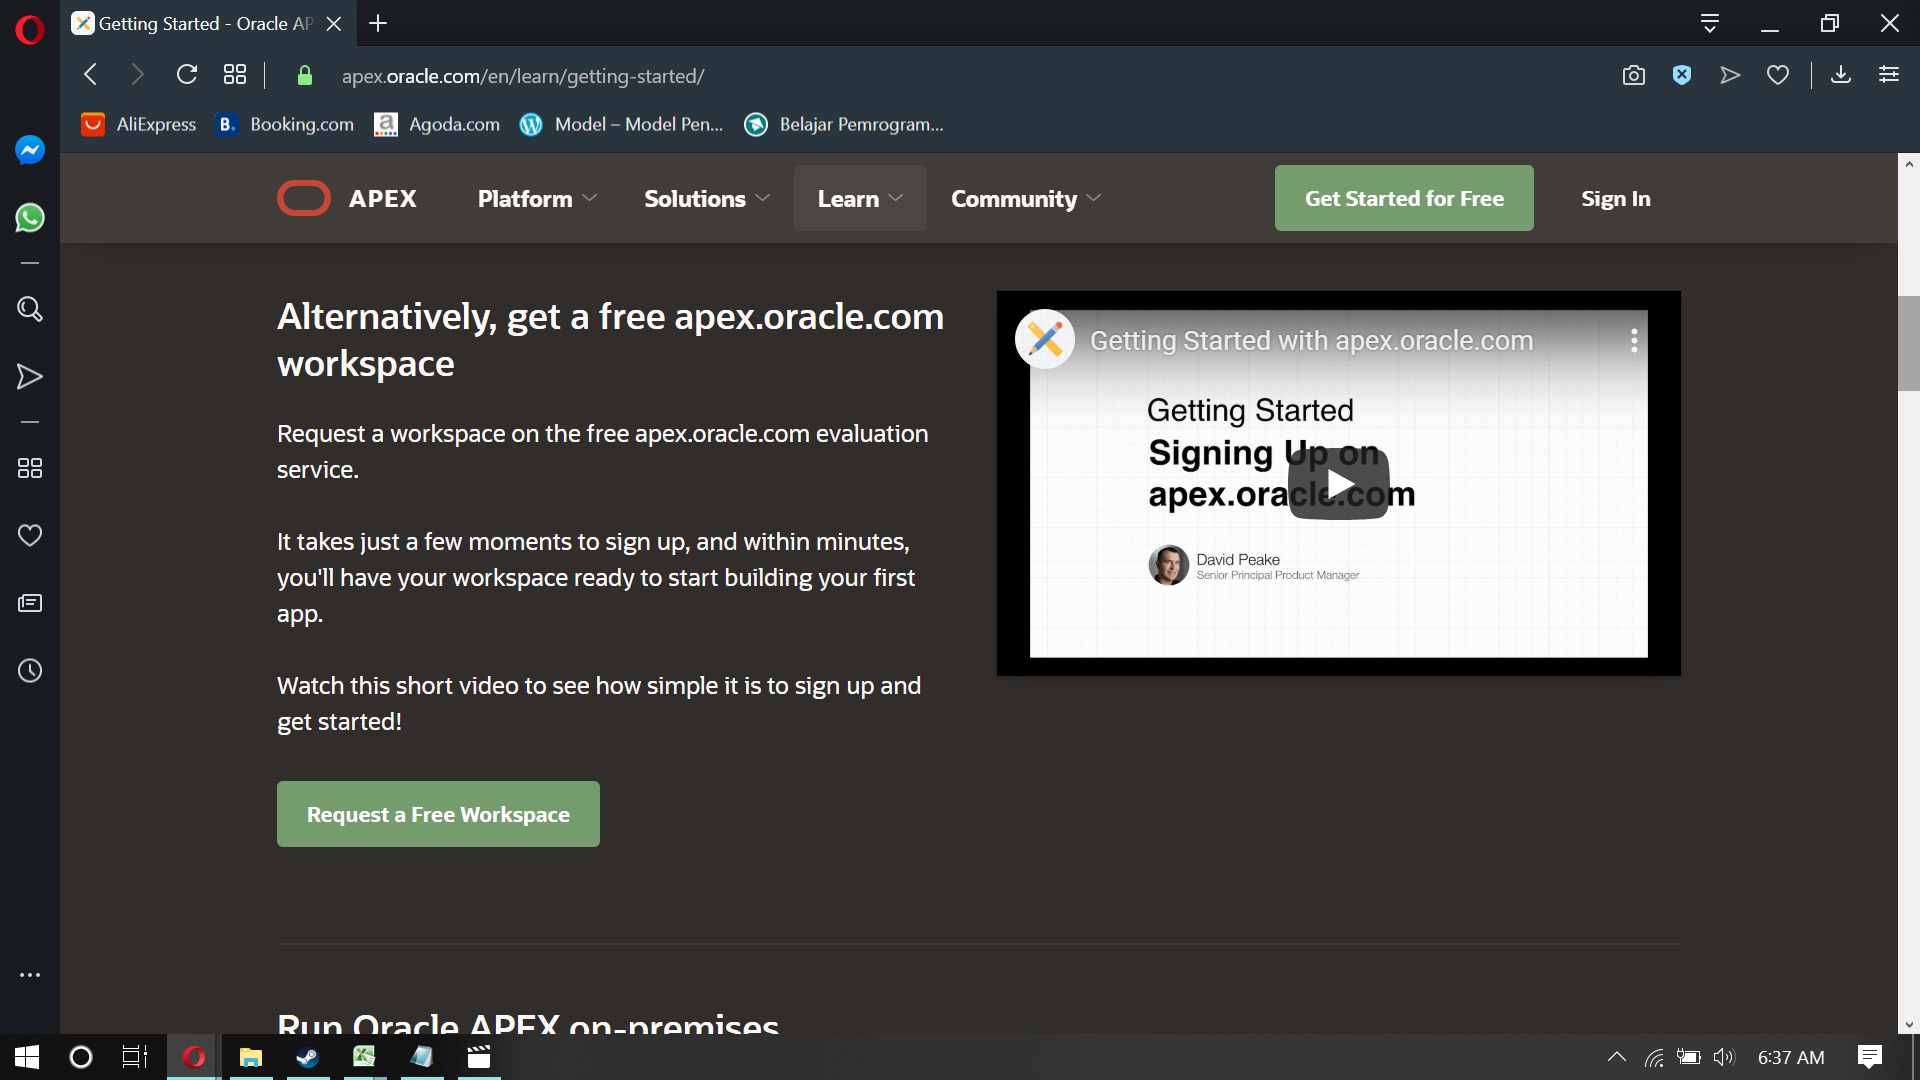
\includegraphics[width=10cm]{gambar/Screenshot (106).png} 
	\item Isi form sesuai dengan yang dibutuhkan, lalu klik next\\	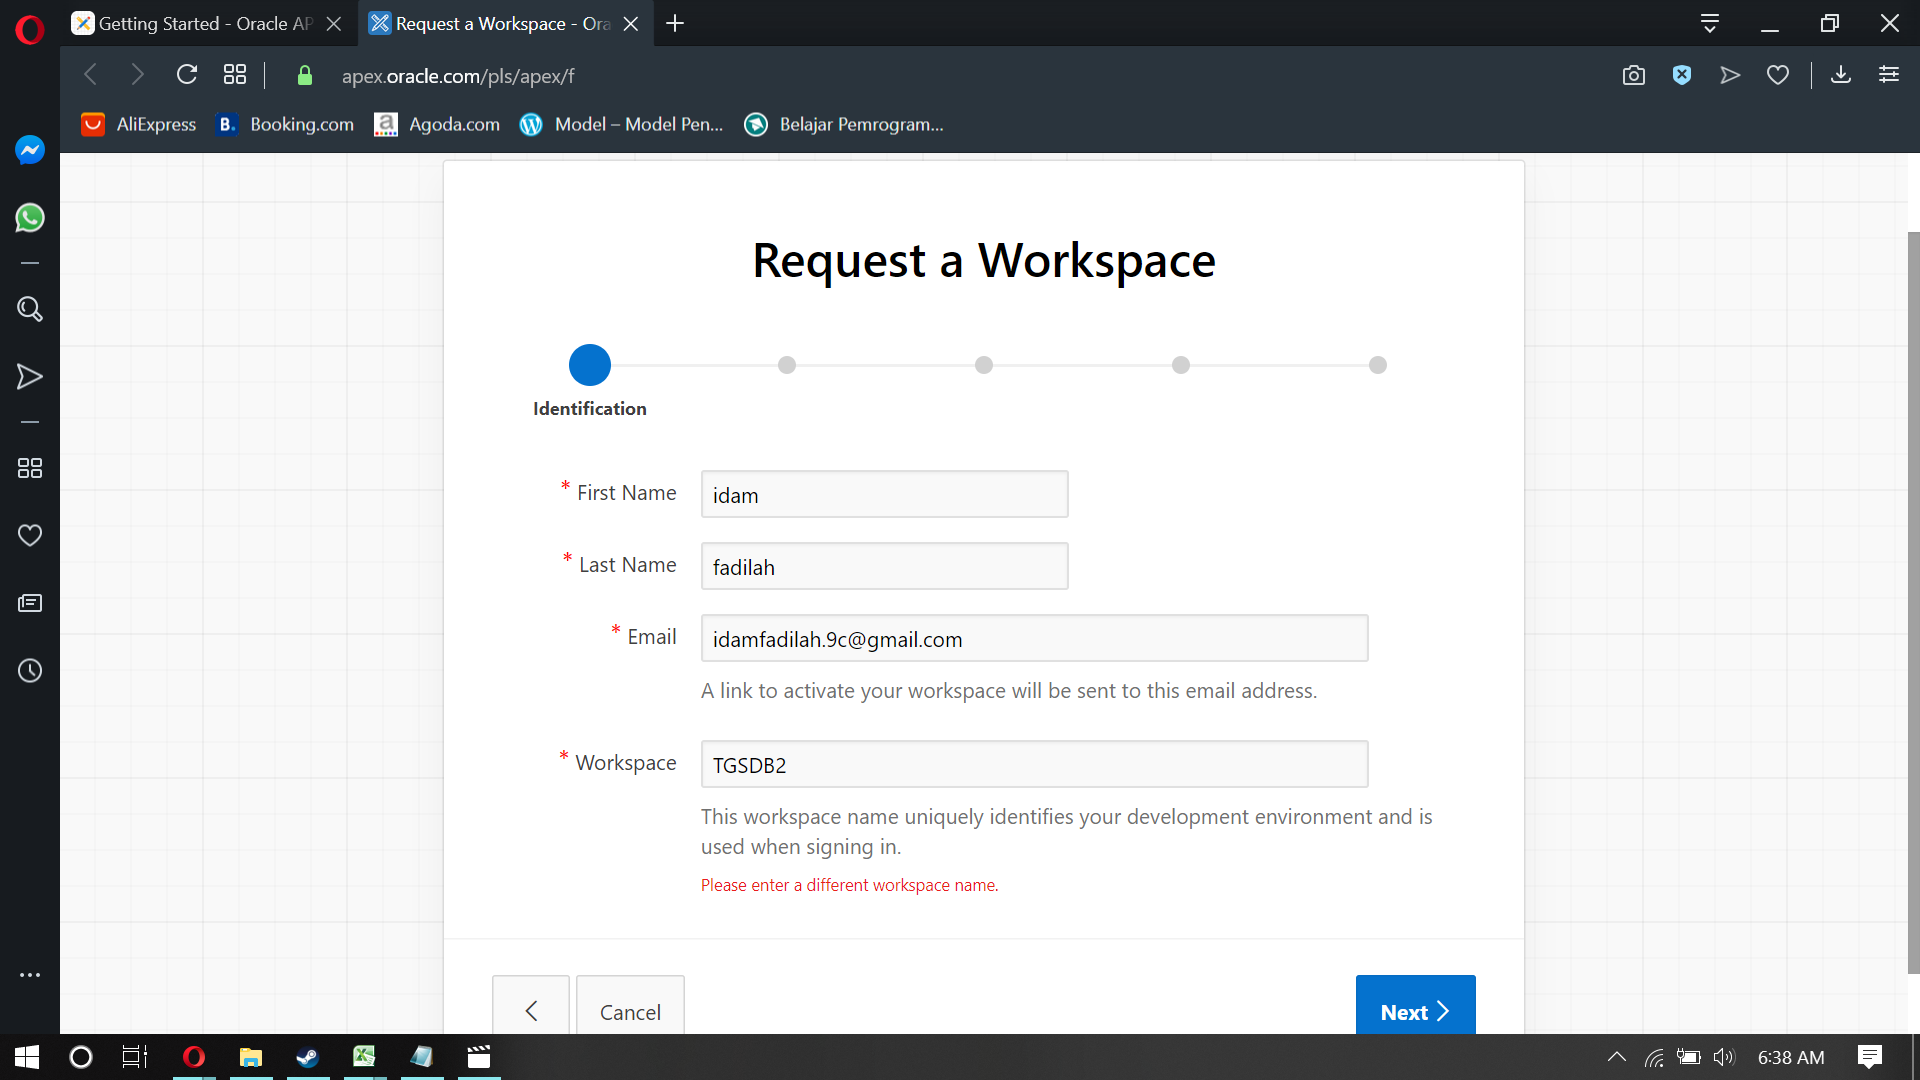
\includegraphics[width=10cm]{gambar/Screenshot (108).png} 
	\item Cetang "yes" pada kedua penyataan, lalu klik next\\	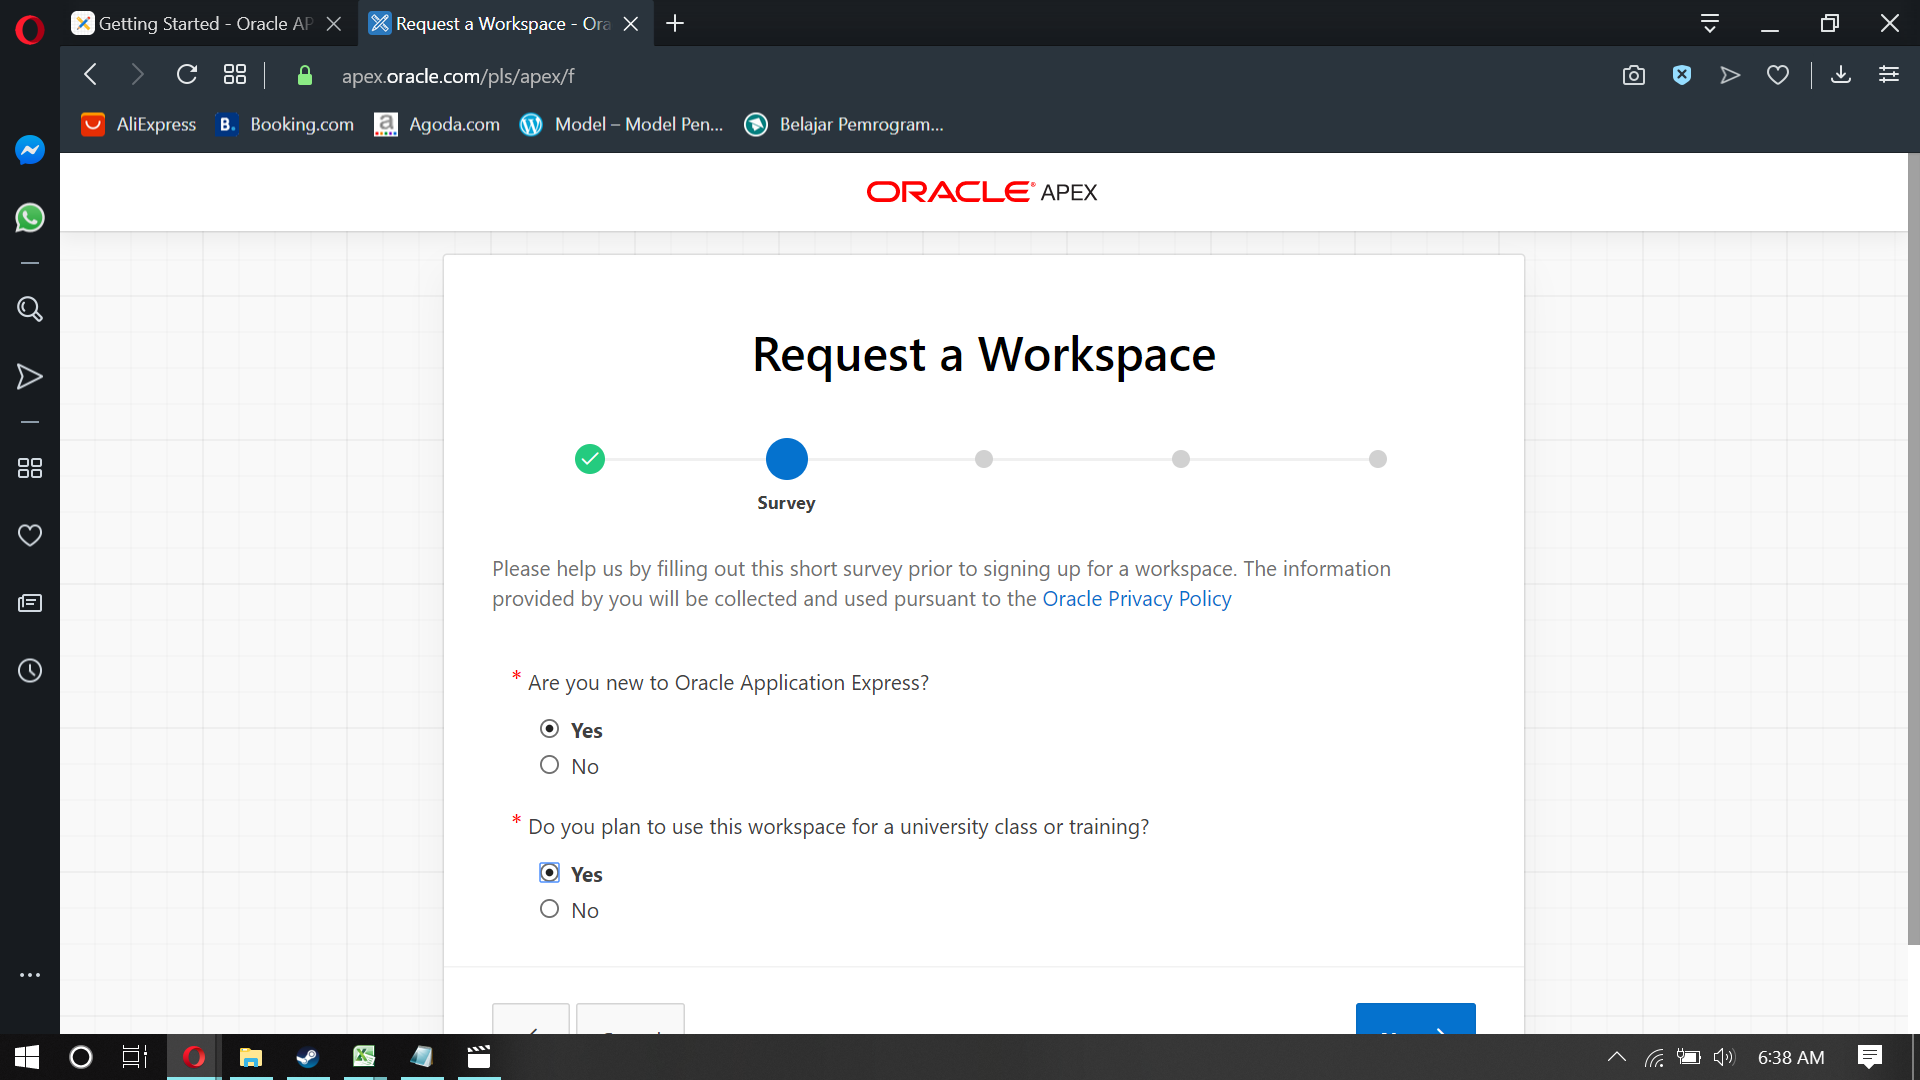
\includegraphics[width=10cm]{gambar/Screenshot (109).png} 
	\item isi form sesuai kebutuhan, lalu klik next\\	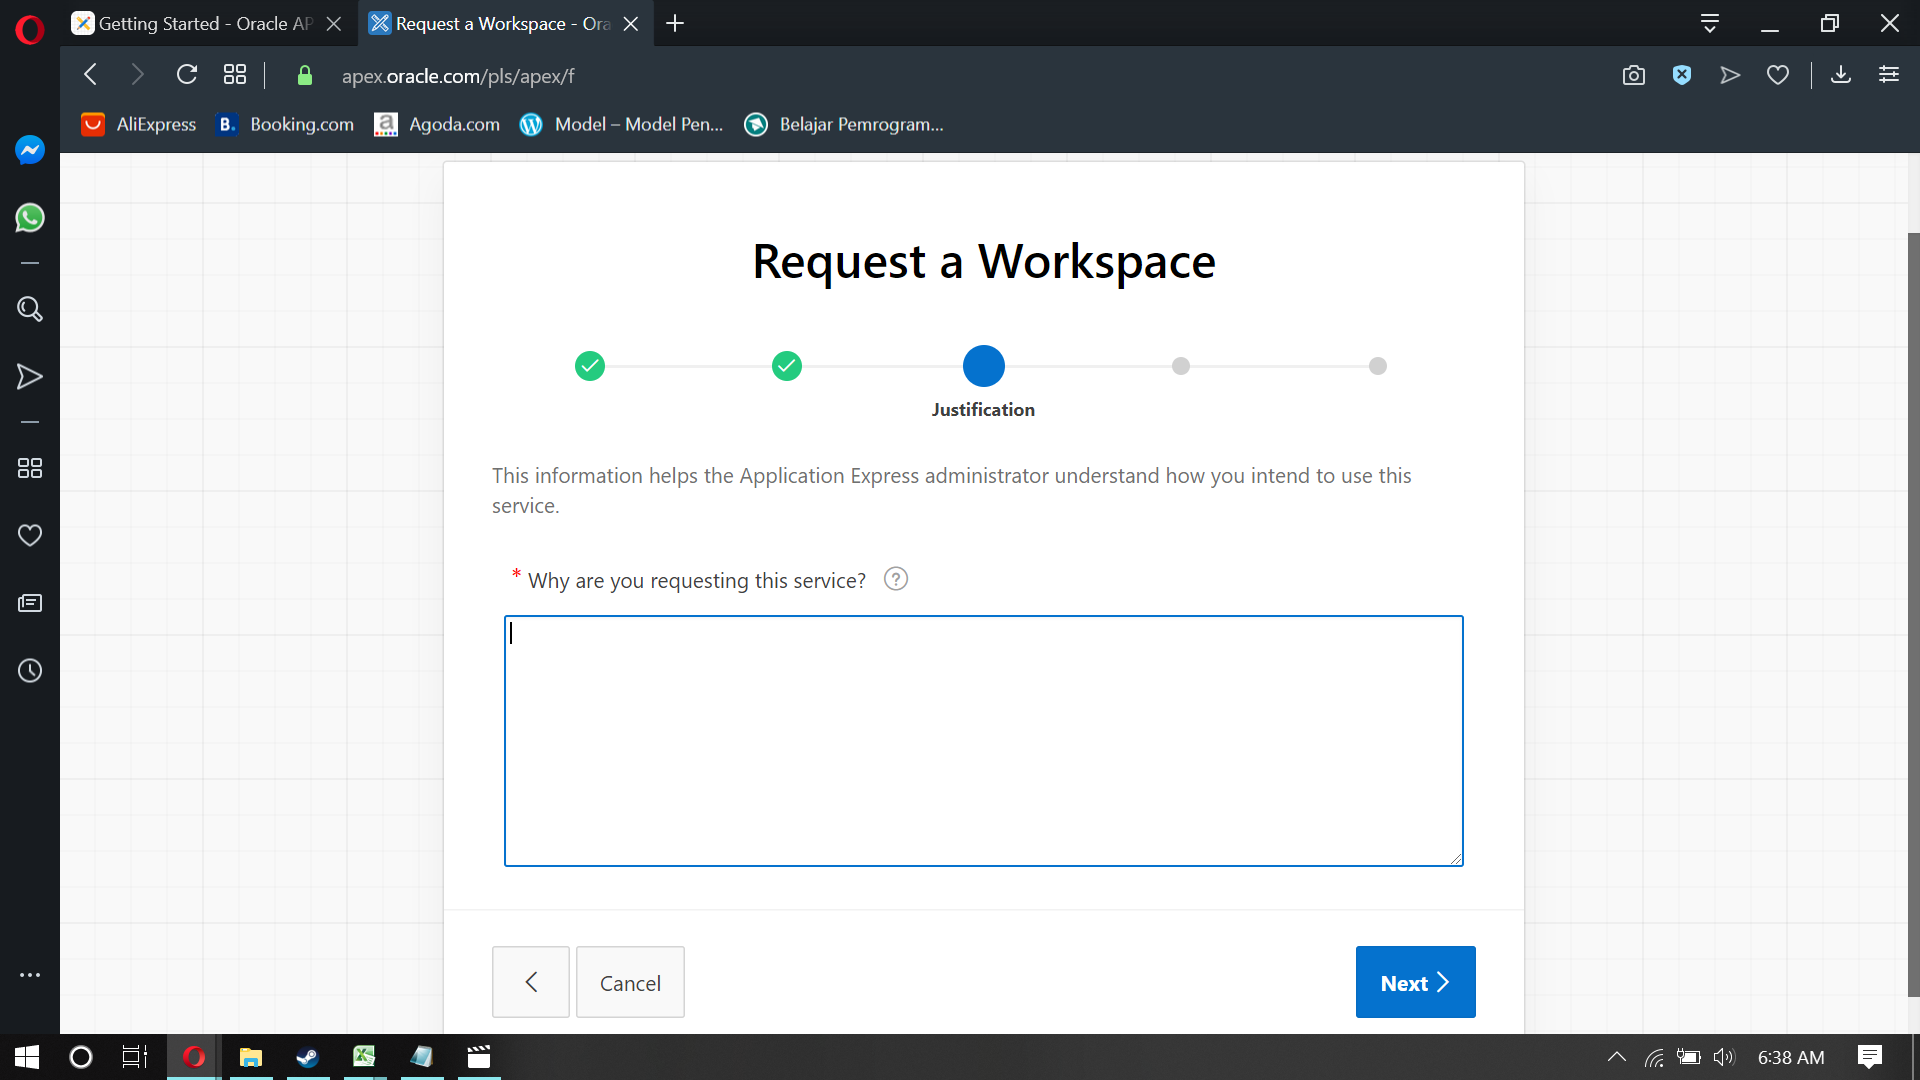
\includegraphics[width=10cm]{gambar/Screenshot (110).png} 
	\item cetang accept, lalu klik next\\	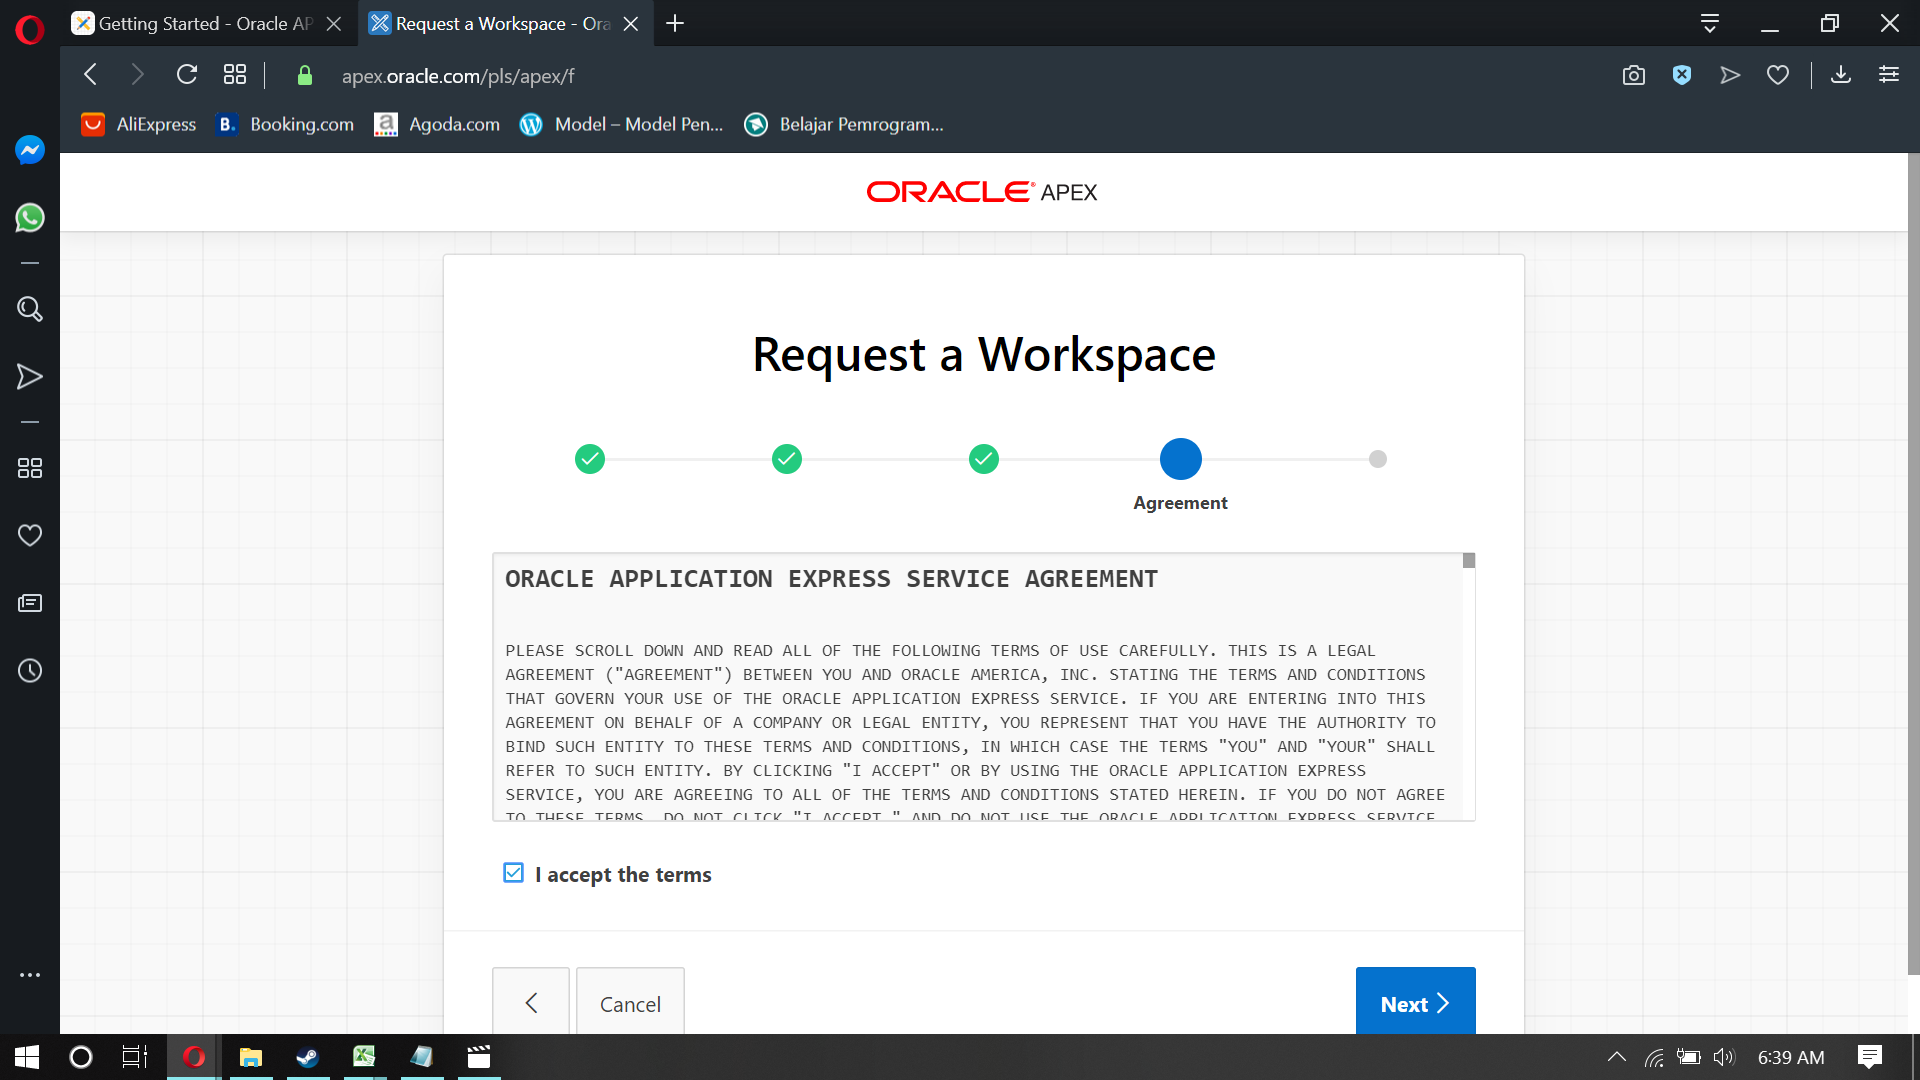
\includegraphics[width=10cm]{gambar/Screenshot (111).png} 
	\item klik submit request\\	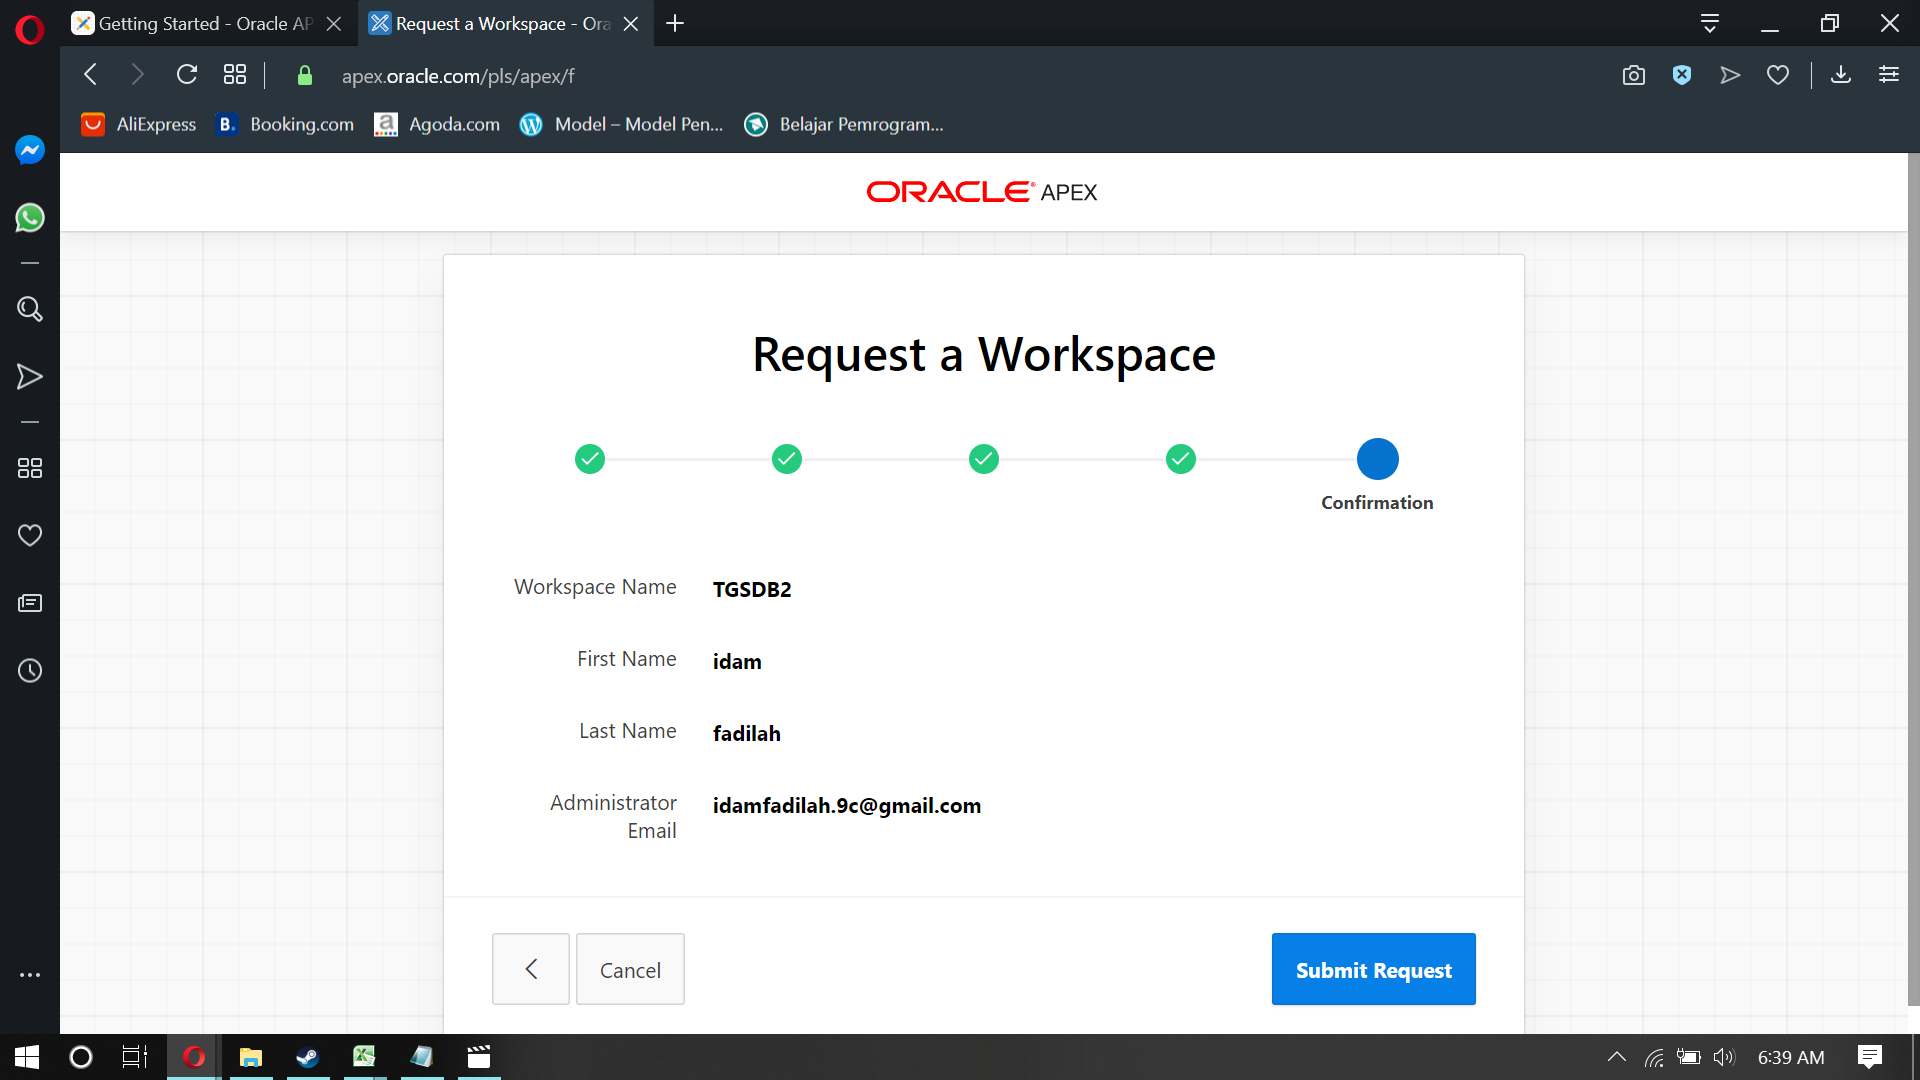
\includegraphics[width=10cm]{gambar/Screenshot (112).png} \\	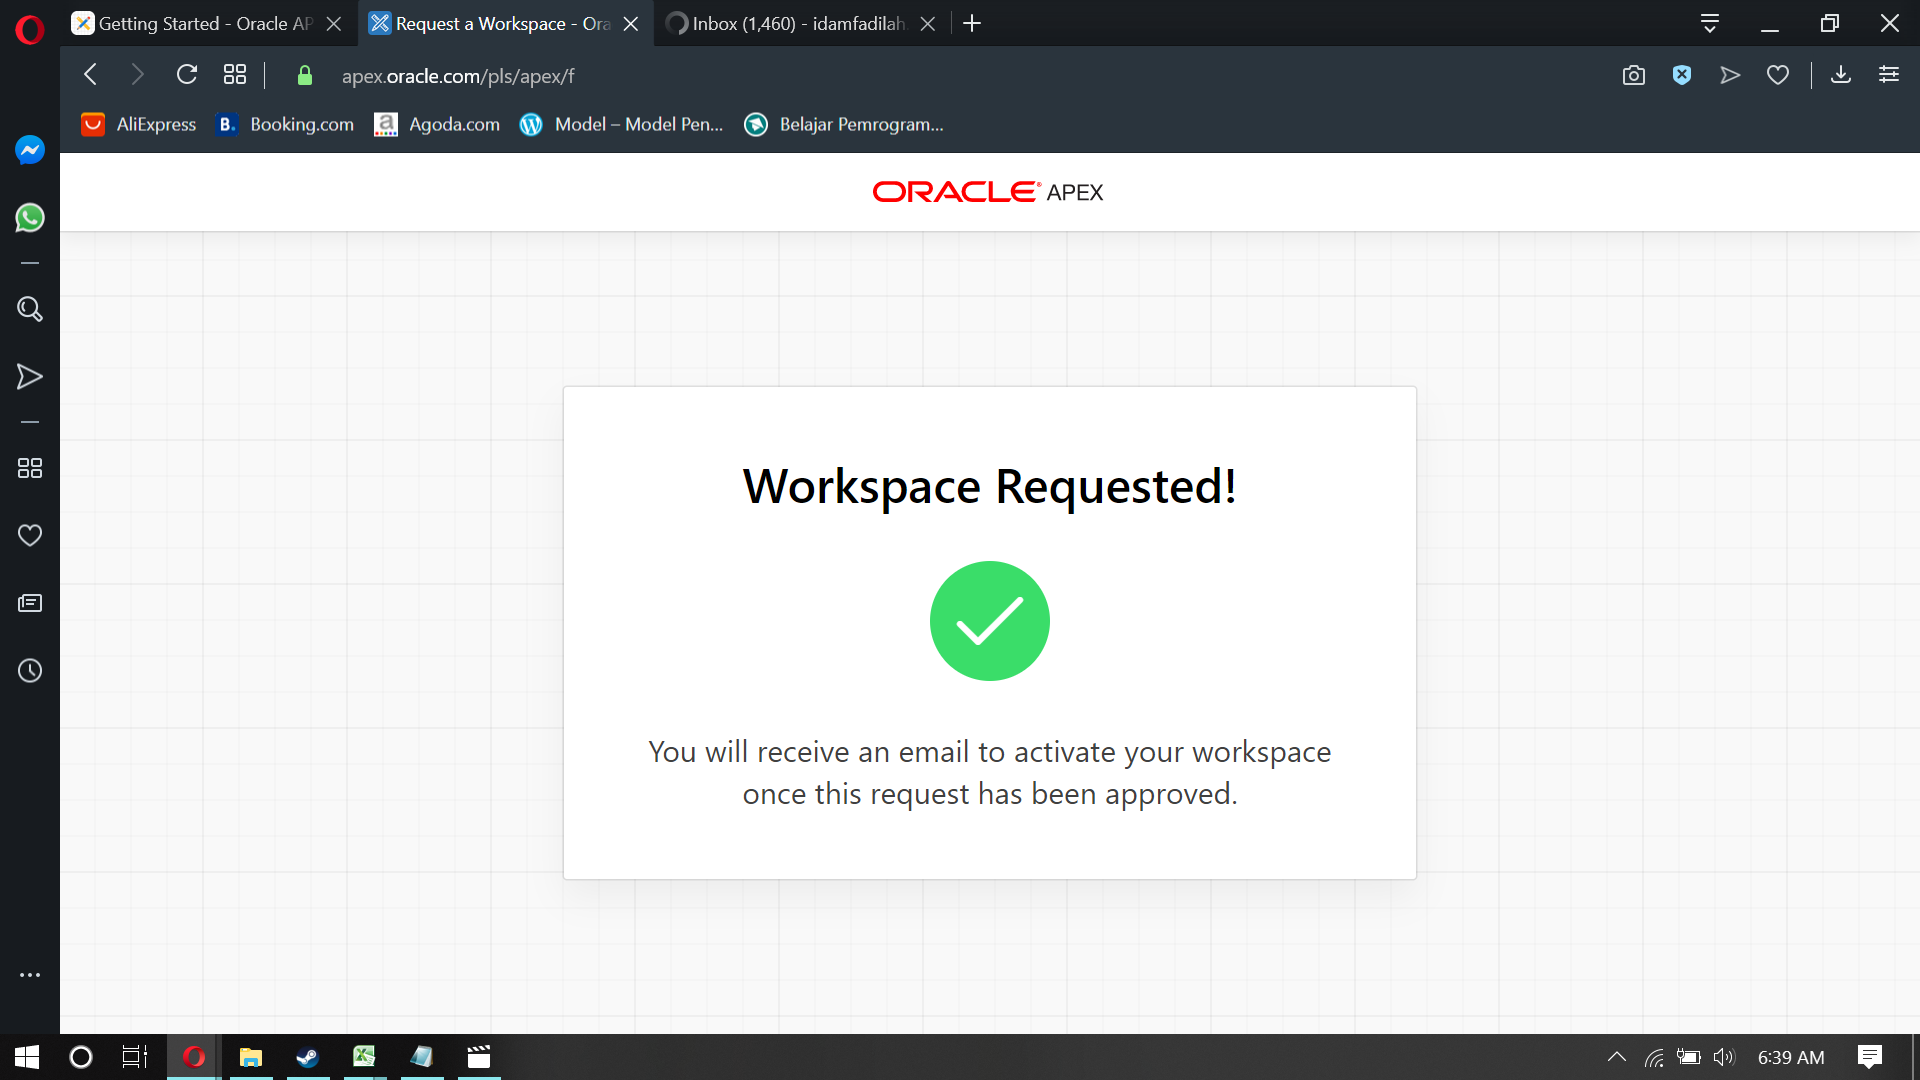
\includegraphics[width=10cm]{gambar/Screenshot (113).png} 
	\item buka email dari oracle lalu klik create workspace\\ 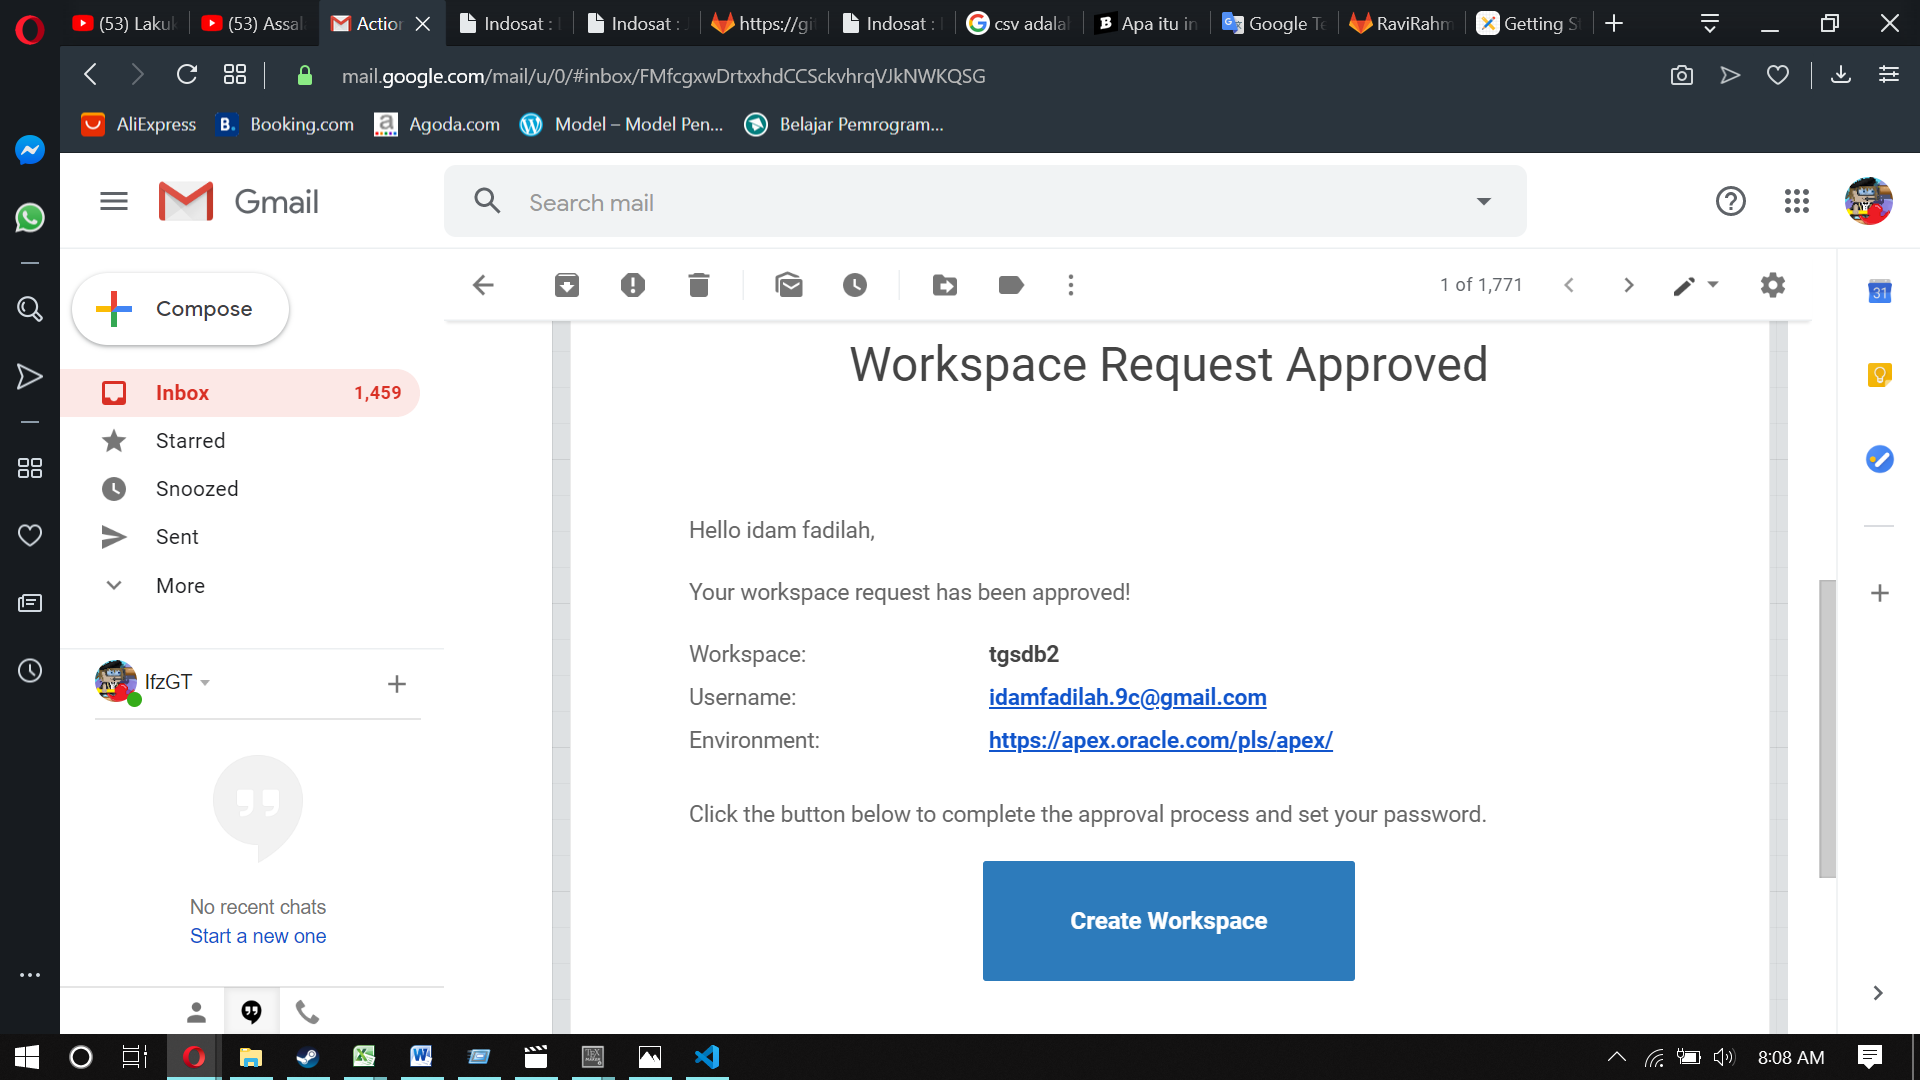
\includegraphics[width=10cm]{gambar/Screenshot (119).png} 
	\item lalu login ke Oracle APEX, dengan data yang sudah didaftarkan\\
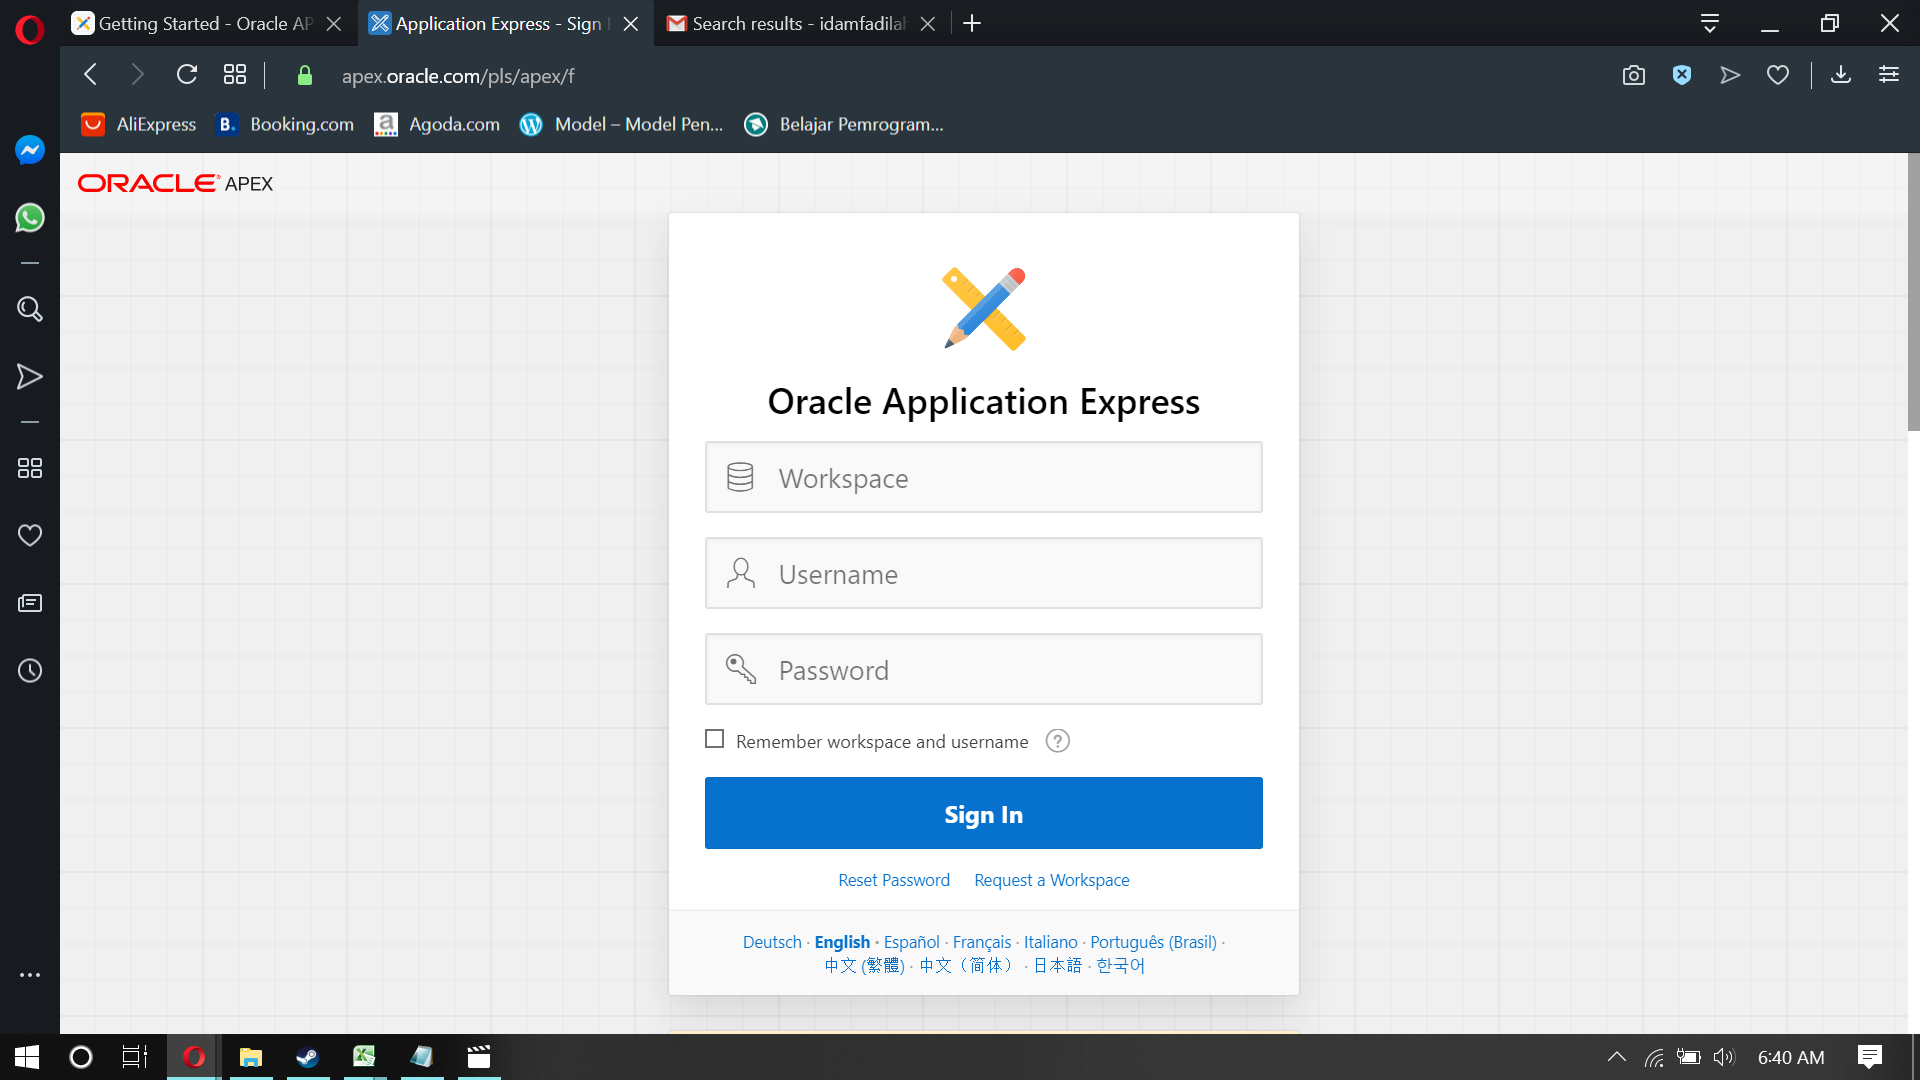
\includegraphics[width=10cm]{gambar/Screenshot (114).png} 
	\item tampilan sesudah login, selesai\\
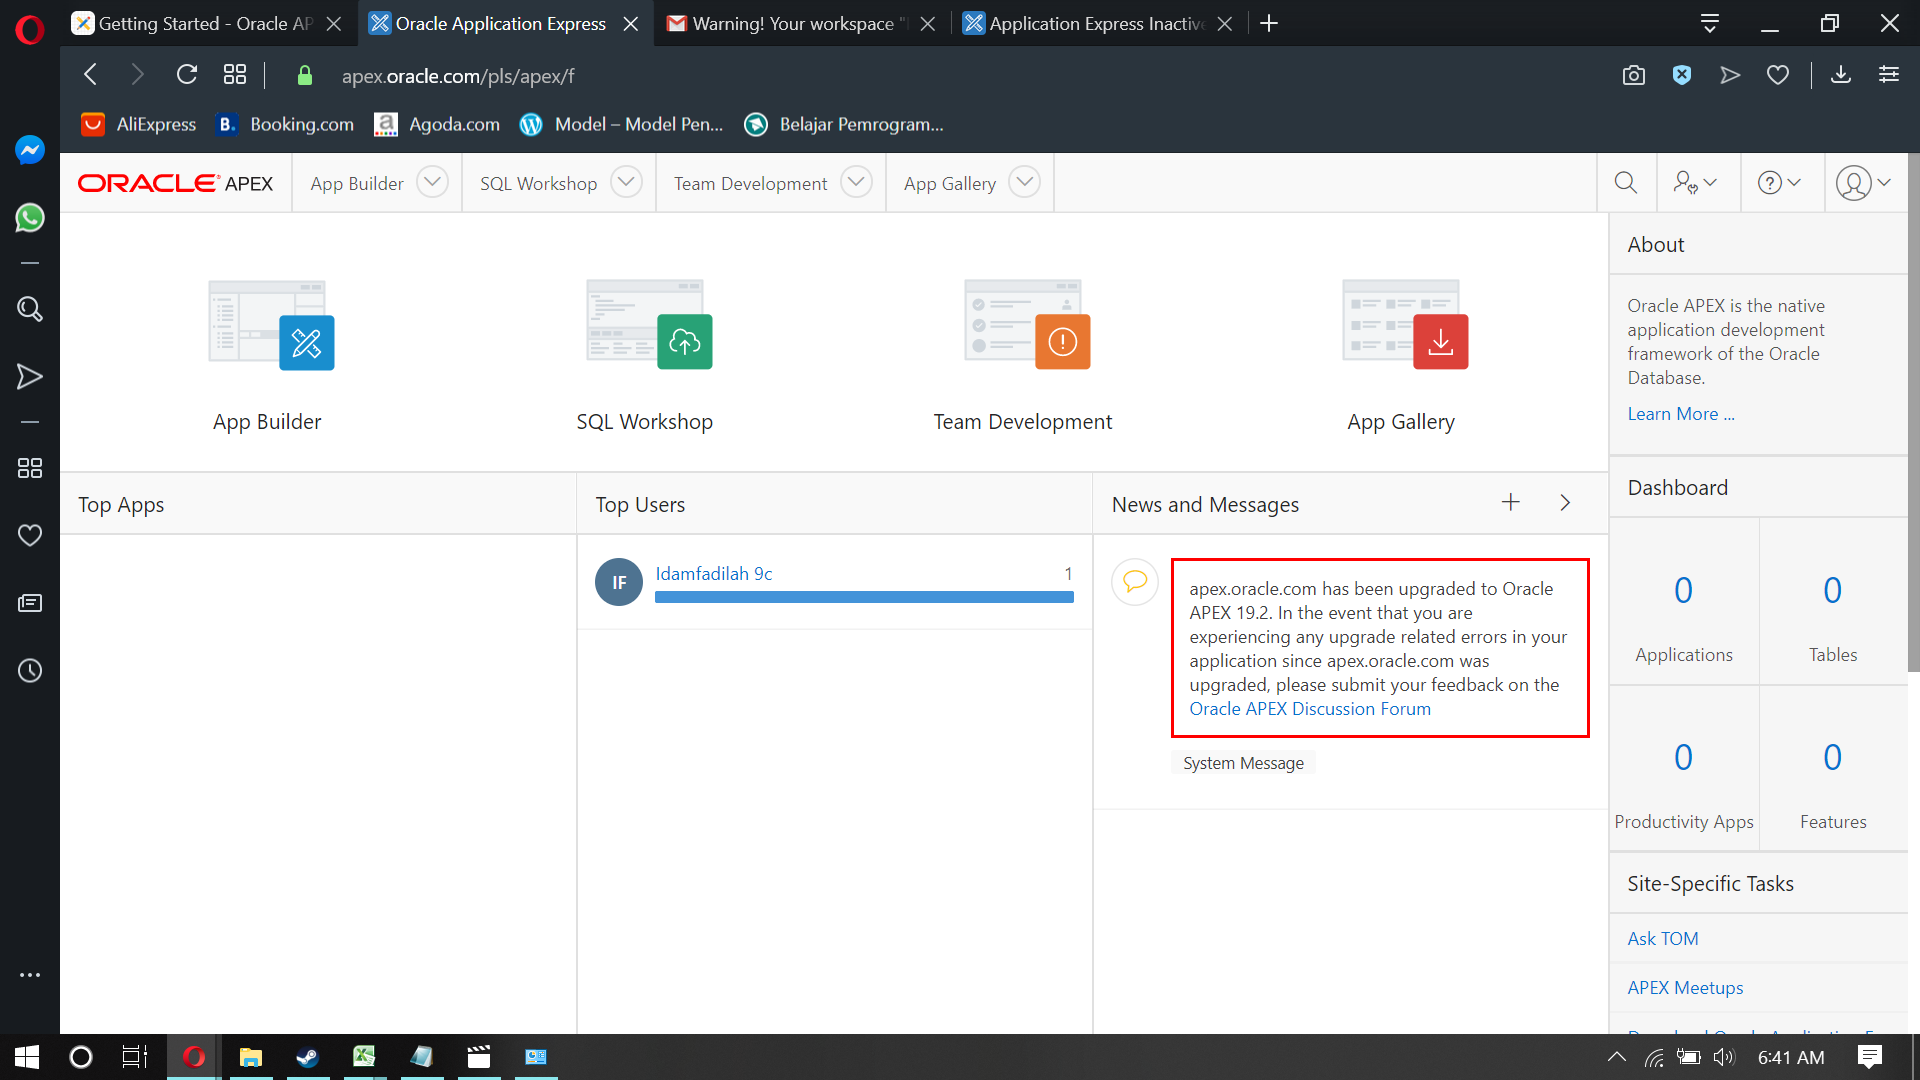
\includegraphics[width=10cm]{gambar/Screenshot (115).png} 
\end{itemize}
\section*{cara membuat table dari data excel}
\paragraph{}
\begin{itemize}
	\item pertama siapkan data excelnya terlebih dahulu, pastikan bahwa kolom paling atas adalah nama kolom yang akan digunakan pada database\\
	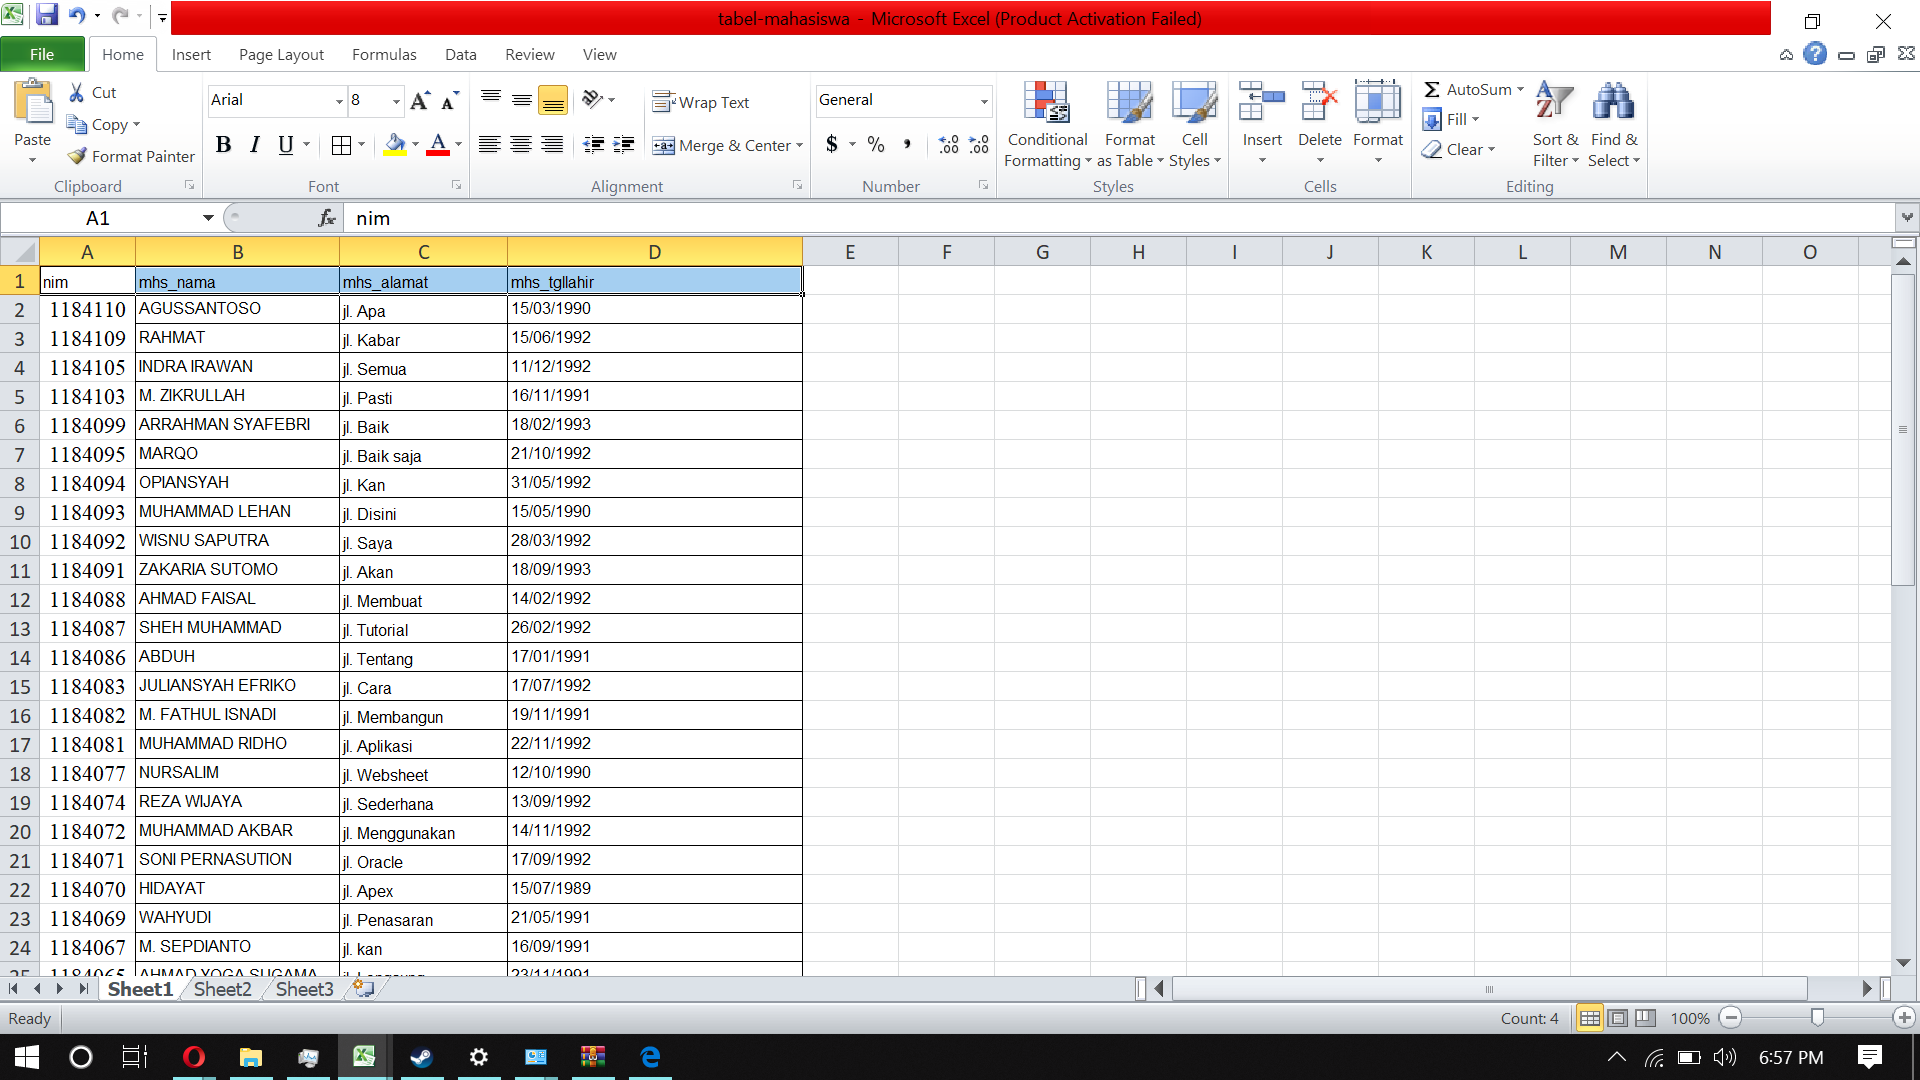
\includegraphics[width=10cm]{excel to db tabel/Screenshot (137).png}\\ 
	\item jika data sudah siap maka masuk ke apex, lalu pilih SQL Workshop/Utilities/Data Workshop\\
	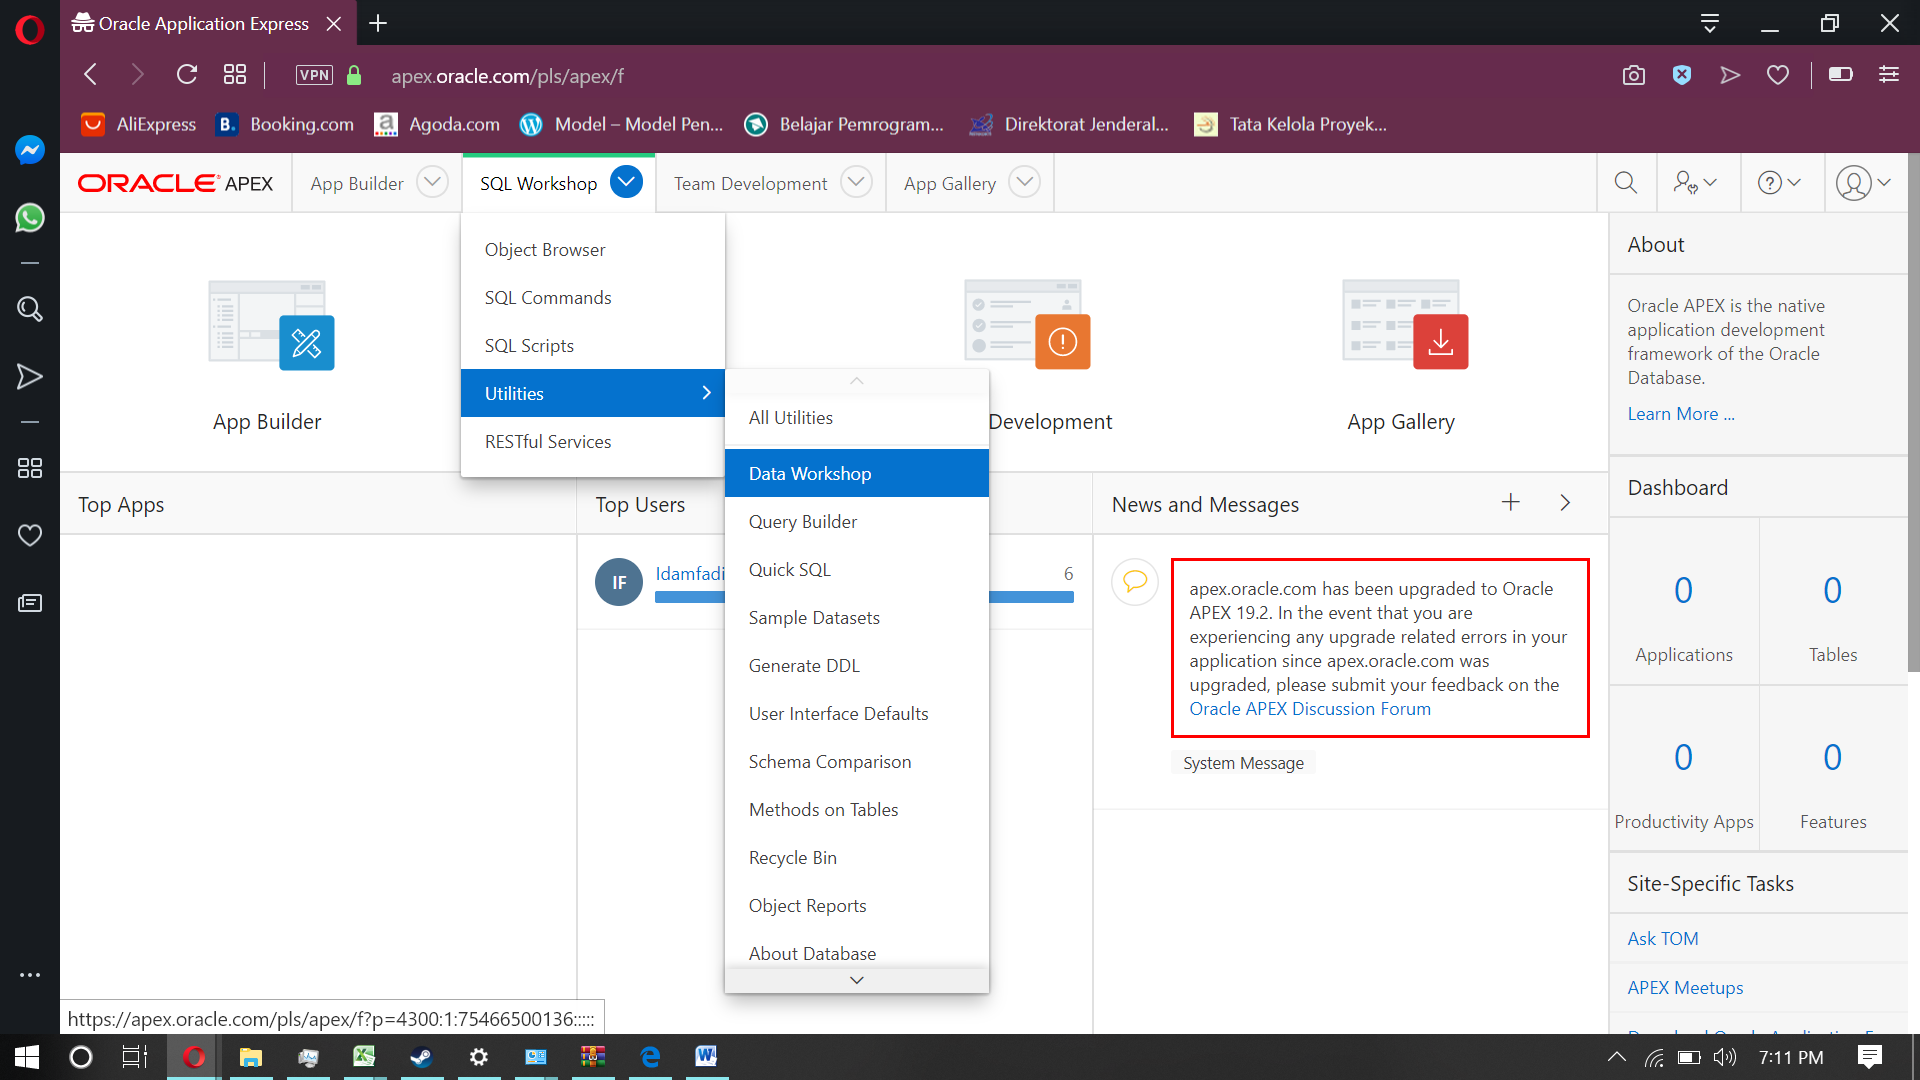
\includegraphics[width=10cm]{excel to db tabel/Screenshot (139).png}\\ 
	\item lalu klik load data\\
	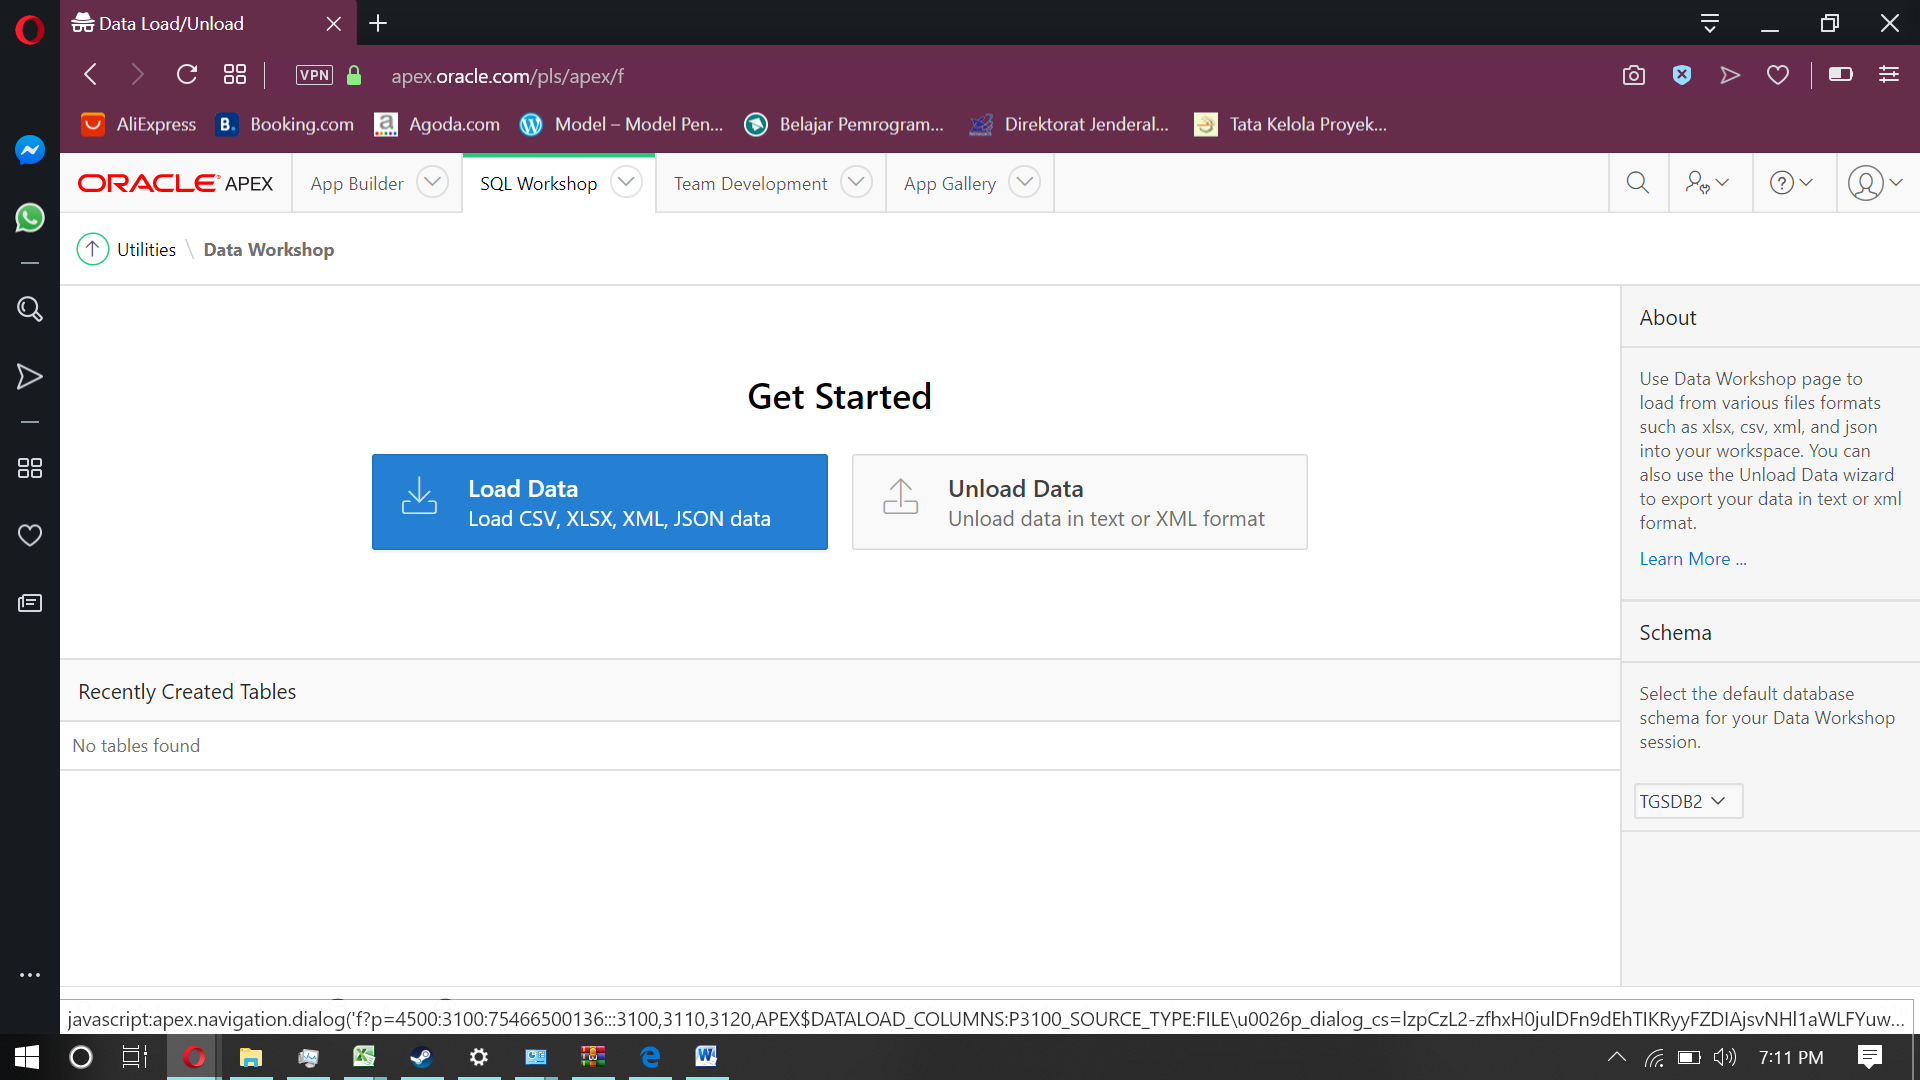
\includegraphics[width=10cm]{excel to db tabel/Screenshot (140).png}\\ 
	\item klik "choose file" atau drag file excel yang sudah disiapkan\\
	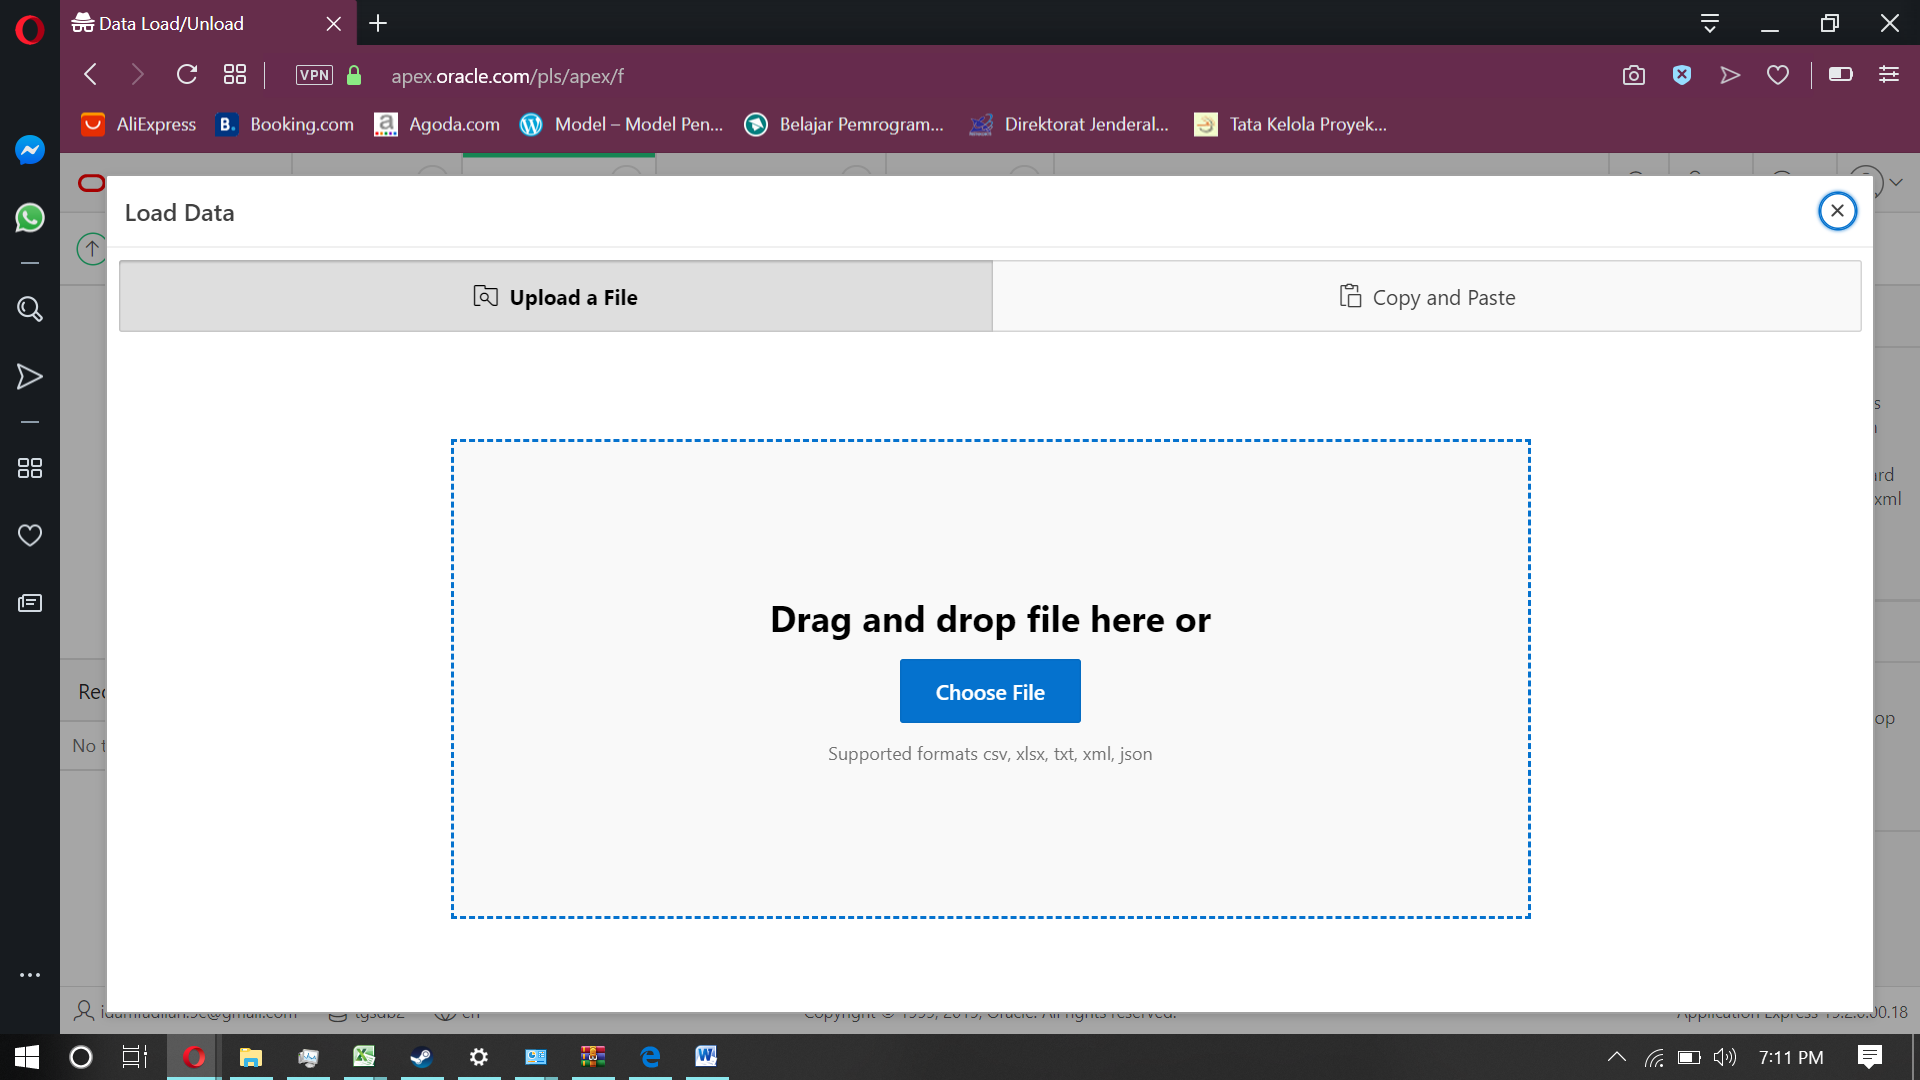
\includegraphics[width=10cm]{excel to db tabel/Screenshot (141).png}\\ 
	\item isi nama tabel, untuk memilih field apa saja yang akan dipakai klik configure\\
	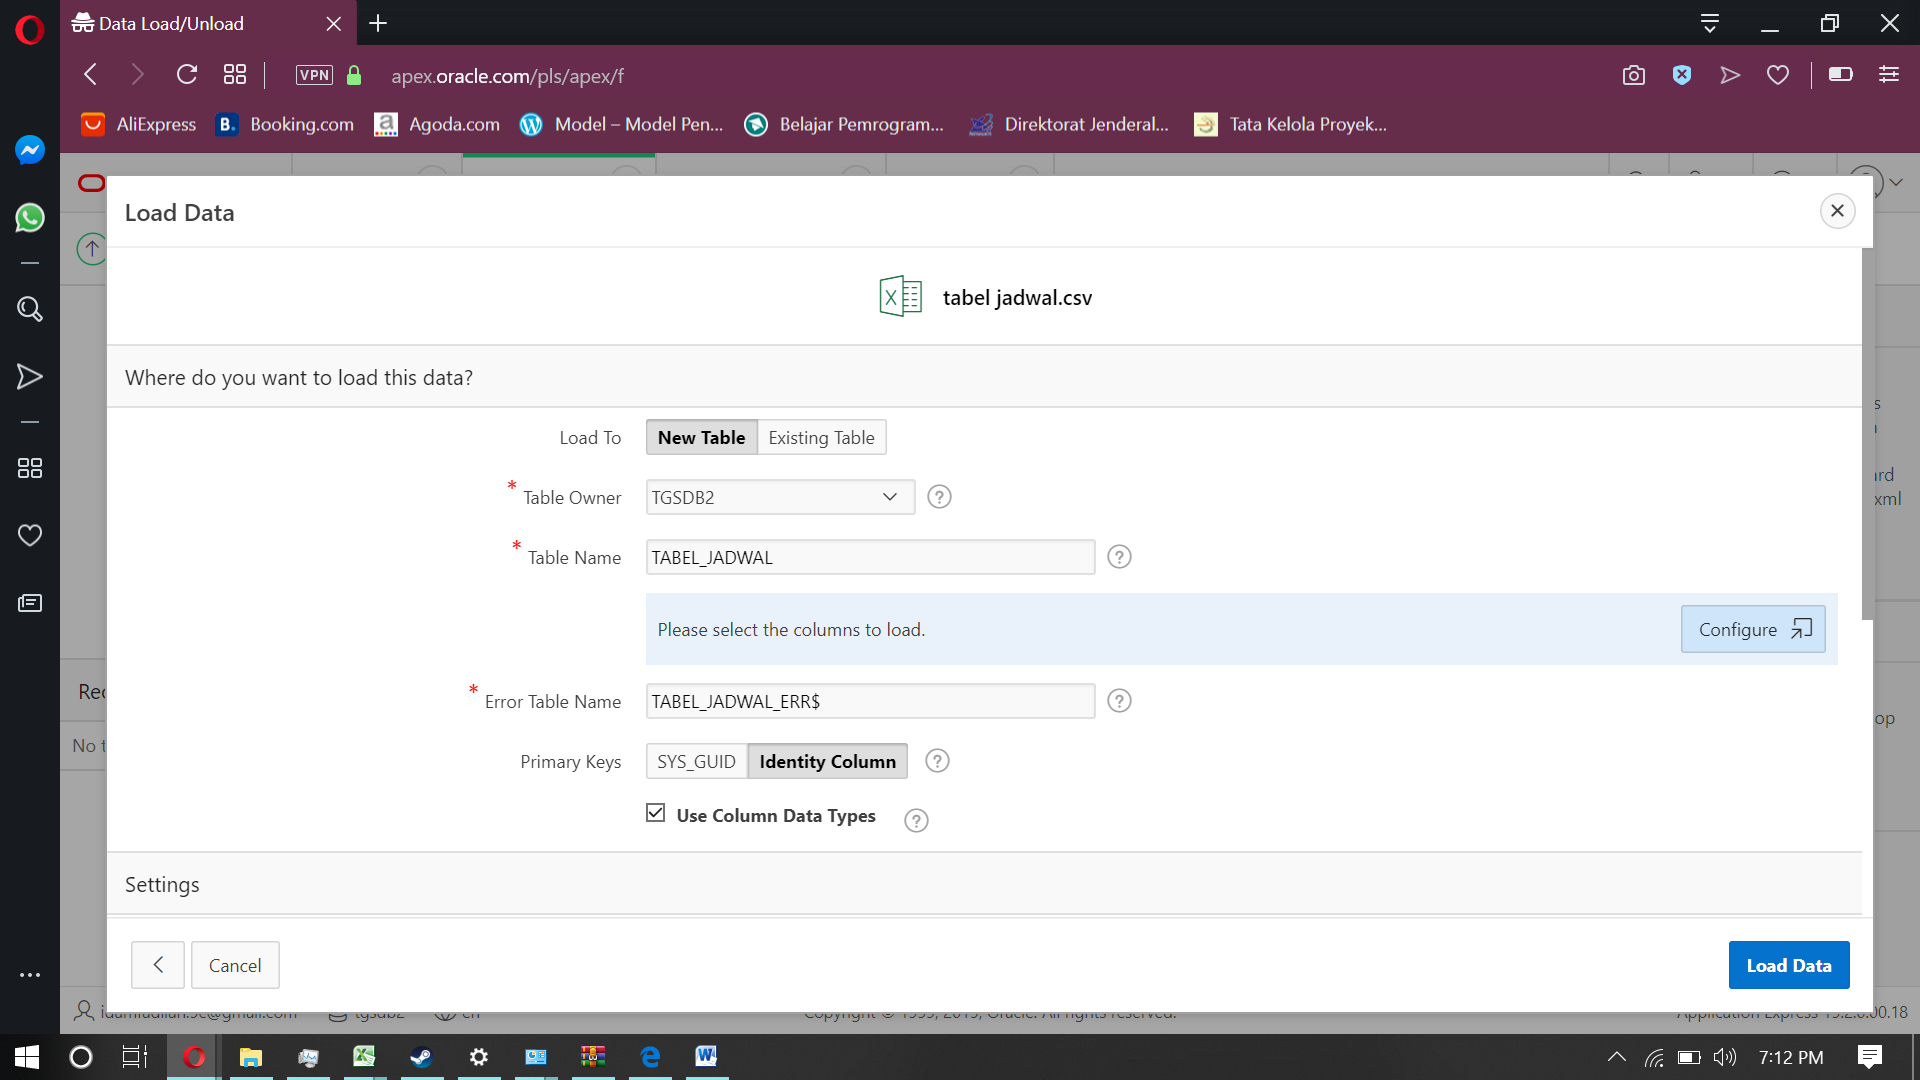
\includegraphics[width=10cm]{excel to db tabel/Screenshot (142).png}\\ 
	\item ceklis field yang diperlukan pada tabel, jika sudah klik "save changes"\\
	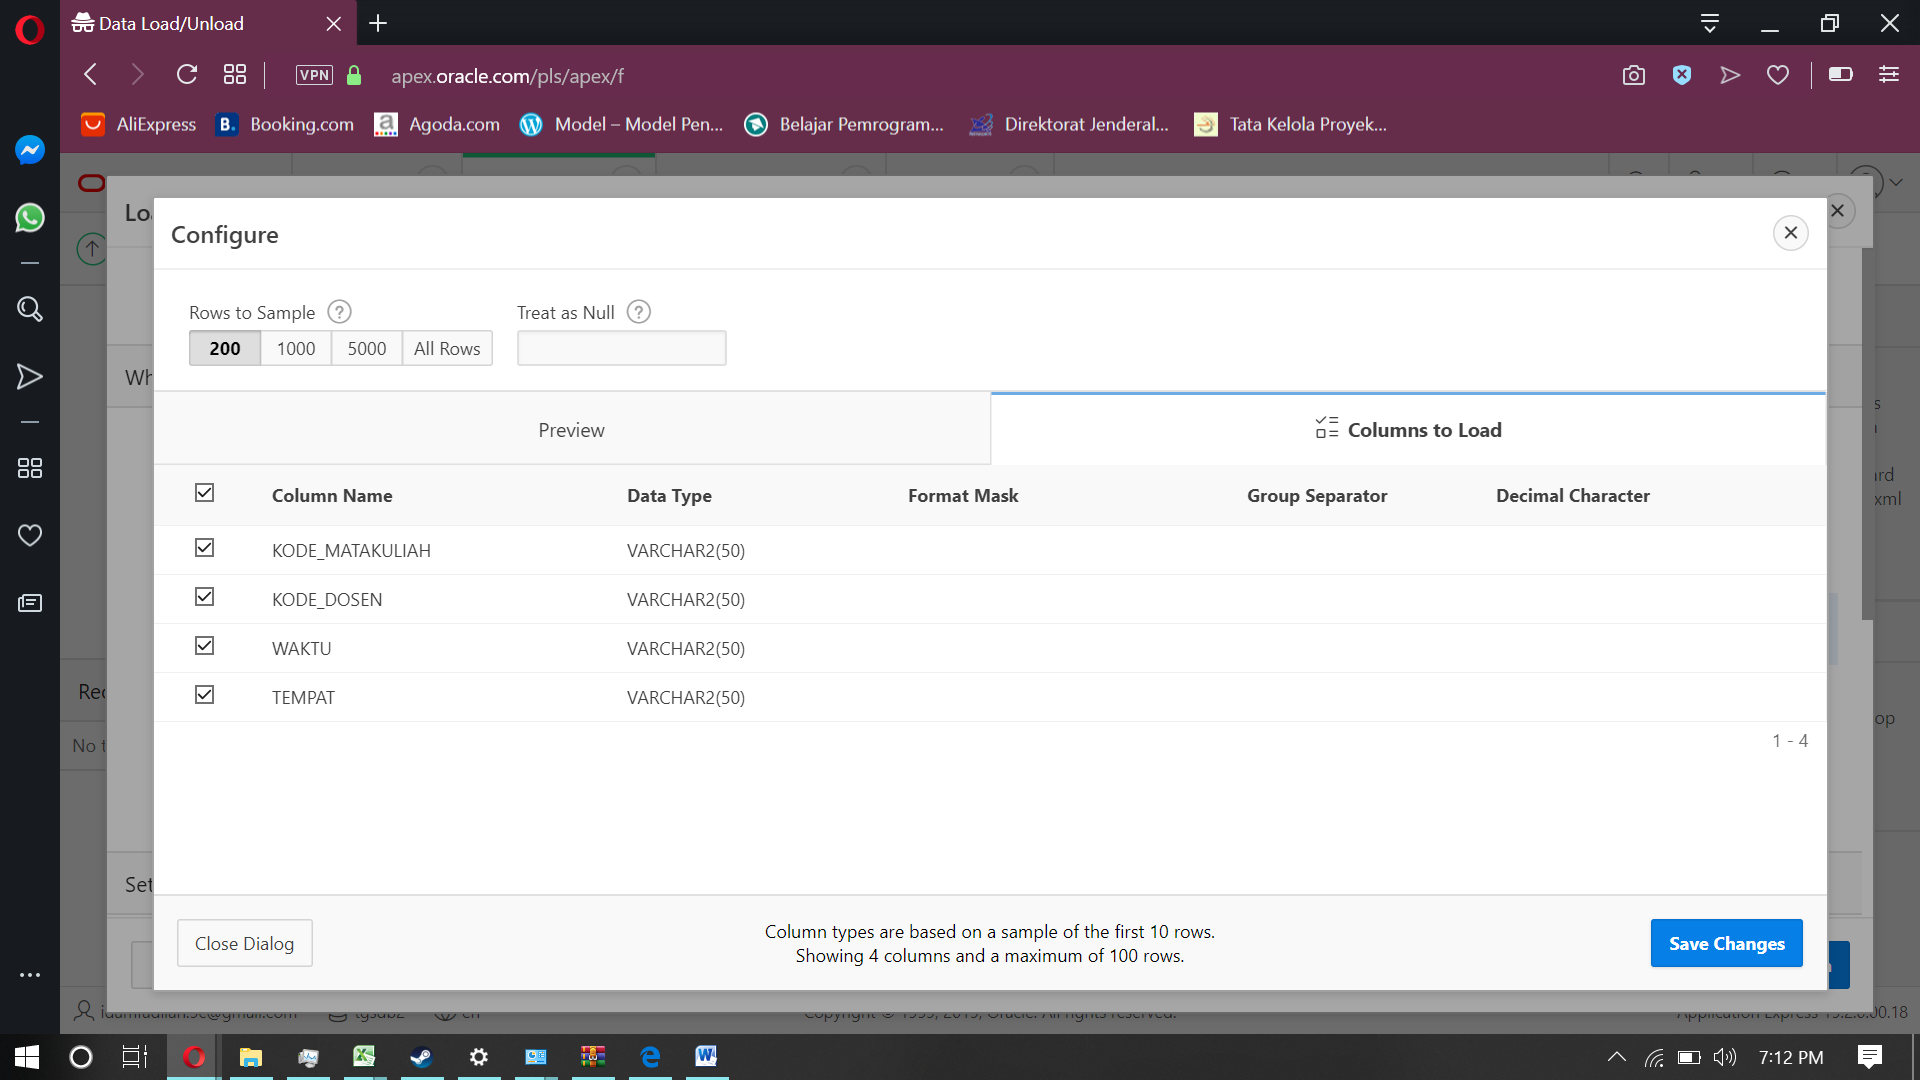
\includegraphics[width=10cm]{excel to db tabel/Screenshot (144).png}\\ 
	\item jika semua telah di konfigurasi maka klik "load data"\\
	

	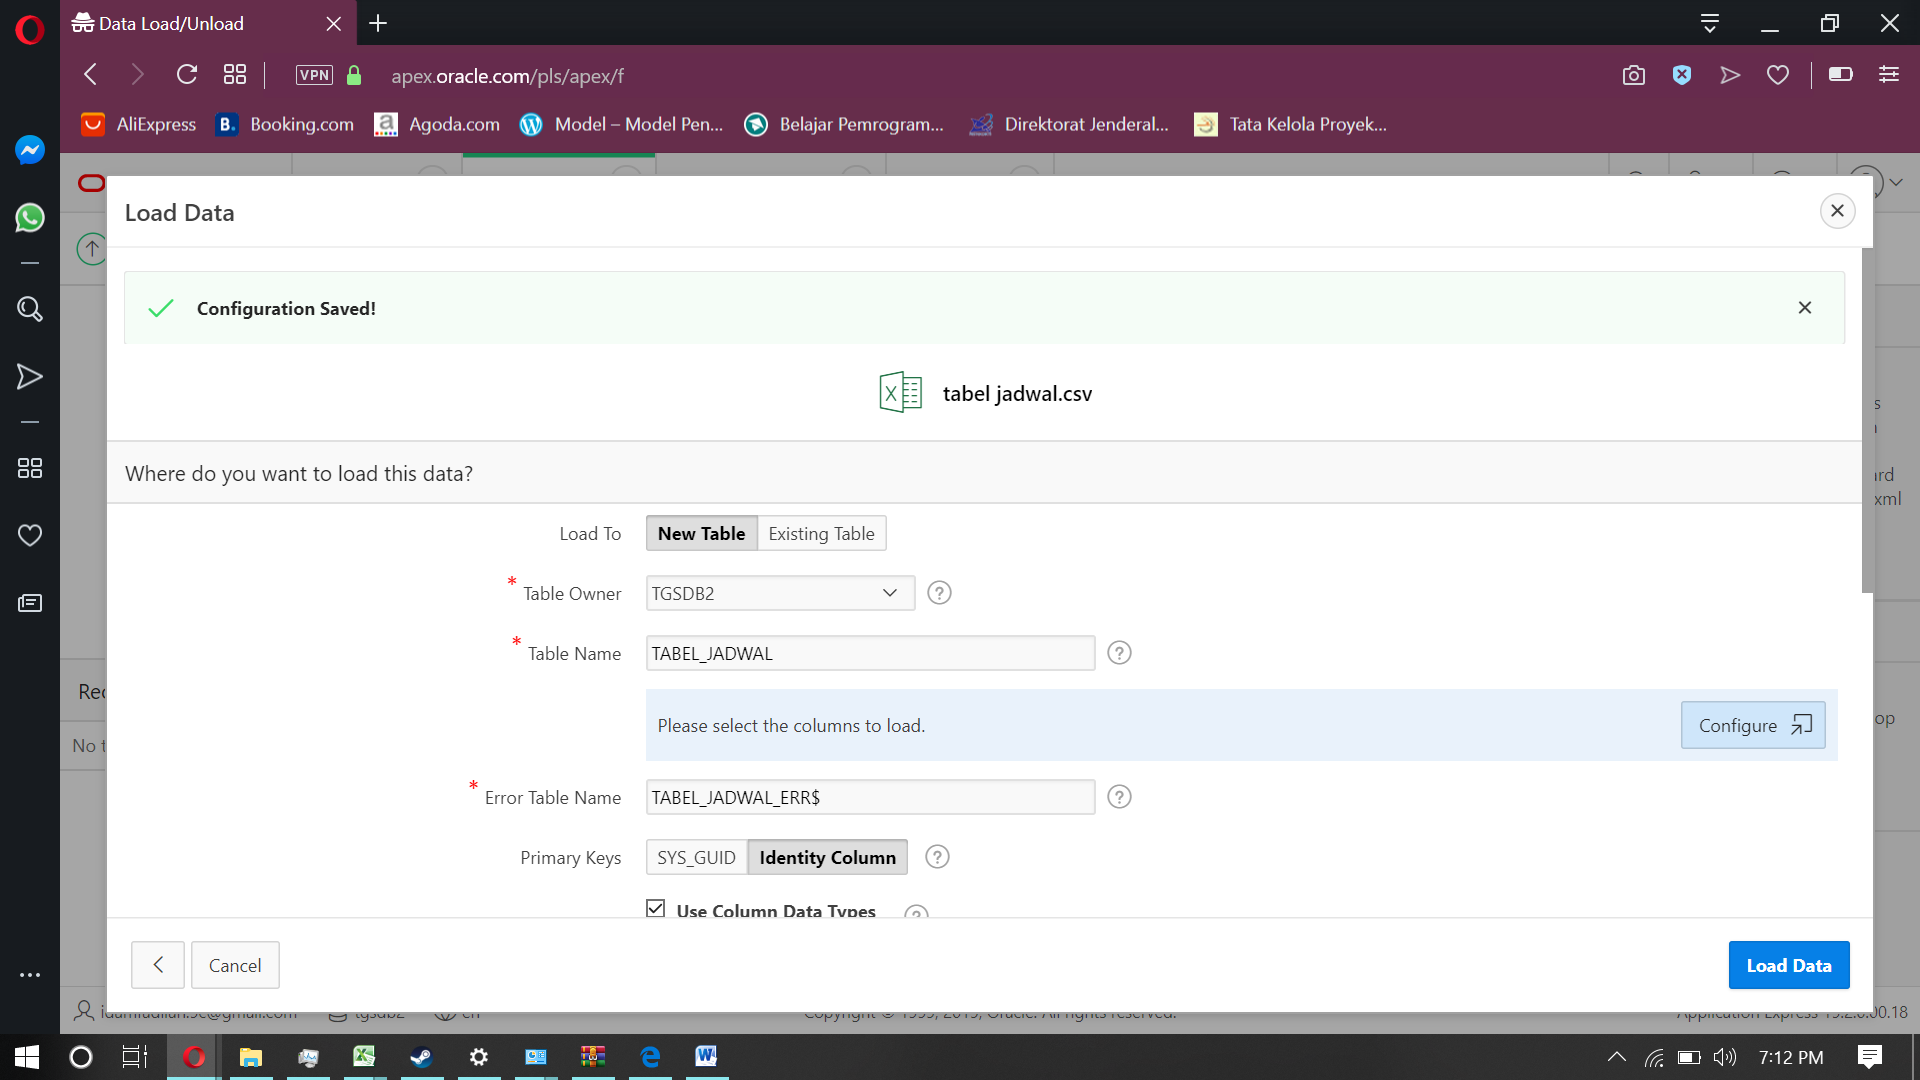
\includegraphics[width=10cm]{excel to db tabel/Screenshot (145).png}\\ 
	\item jika masih ada tabel yang akan di inputkan maka klik tombol (x), jangan dulu create application \\
	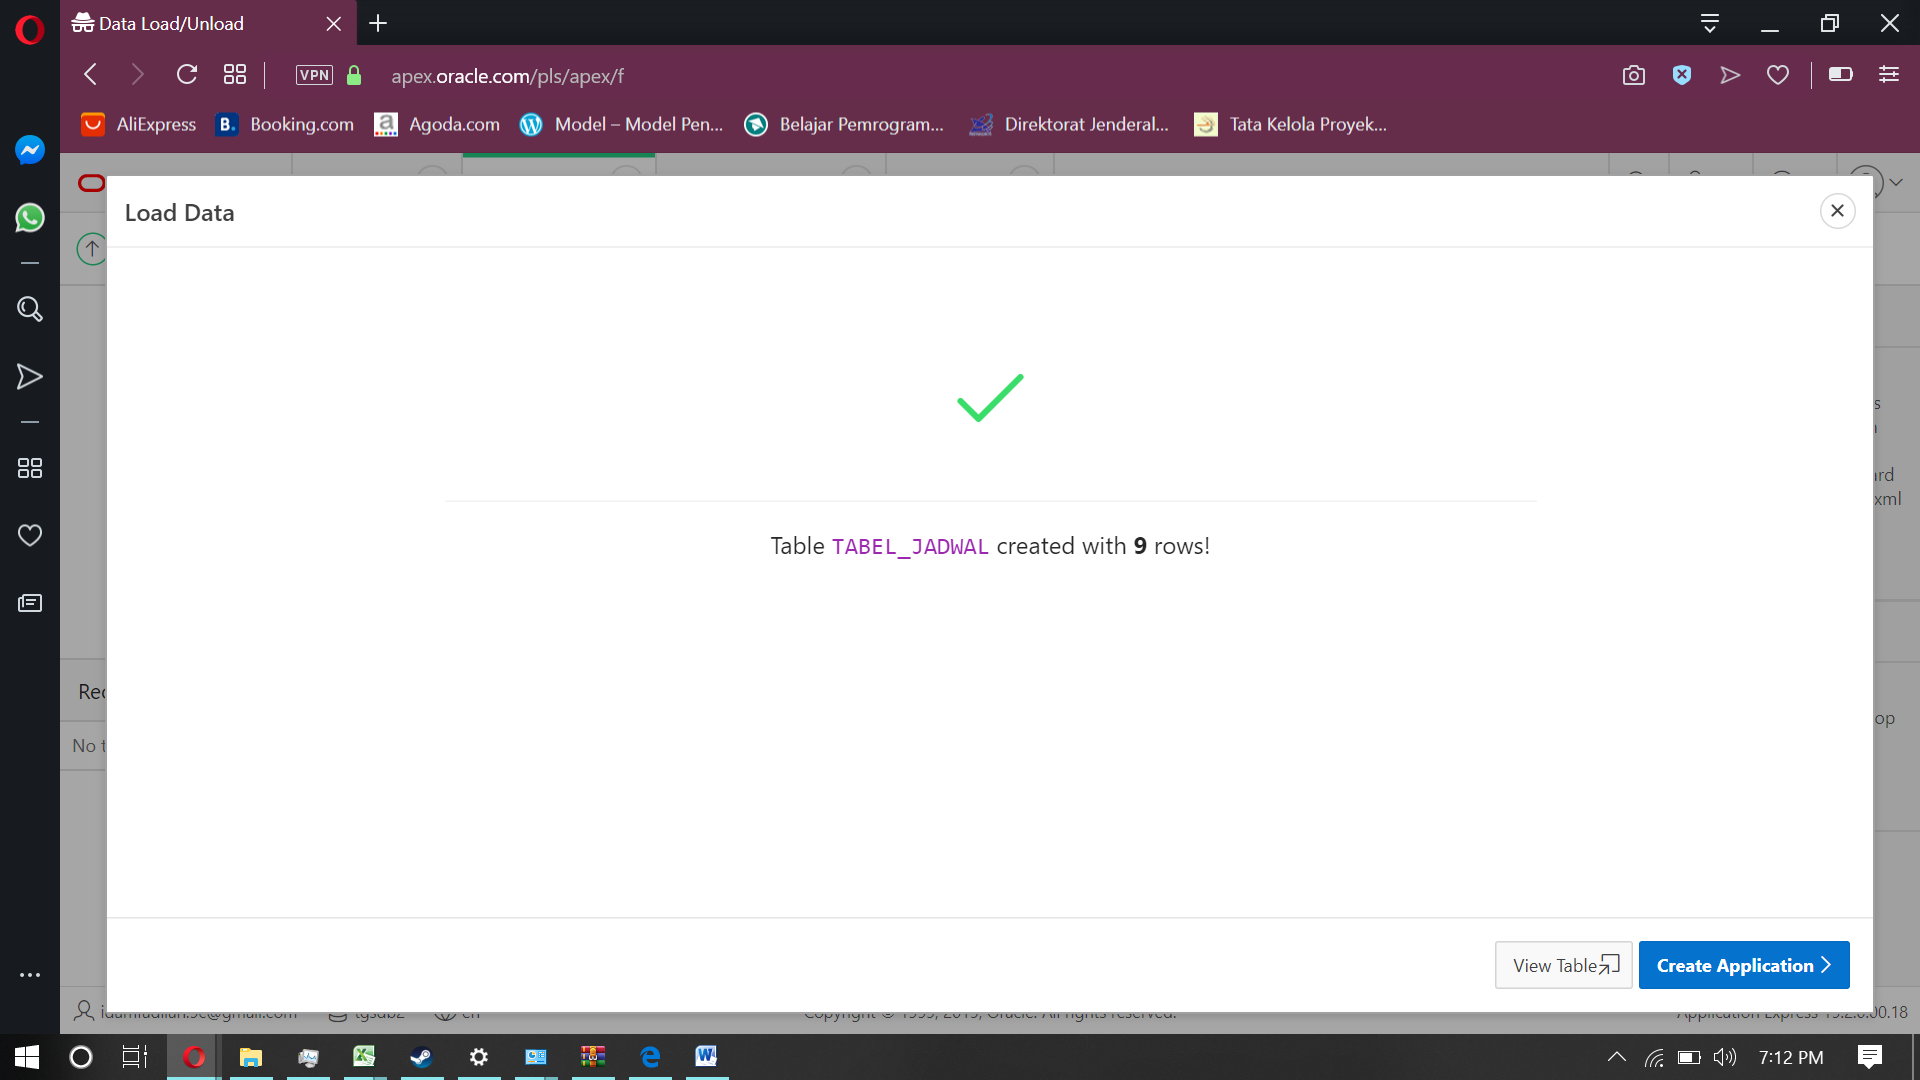
\includegraphics[width=10cm]{excel to db tabel/Screenshot (146).png}\\ 
	\item disini saya membuat telah membuat 5 tabel\\
	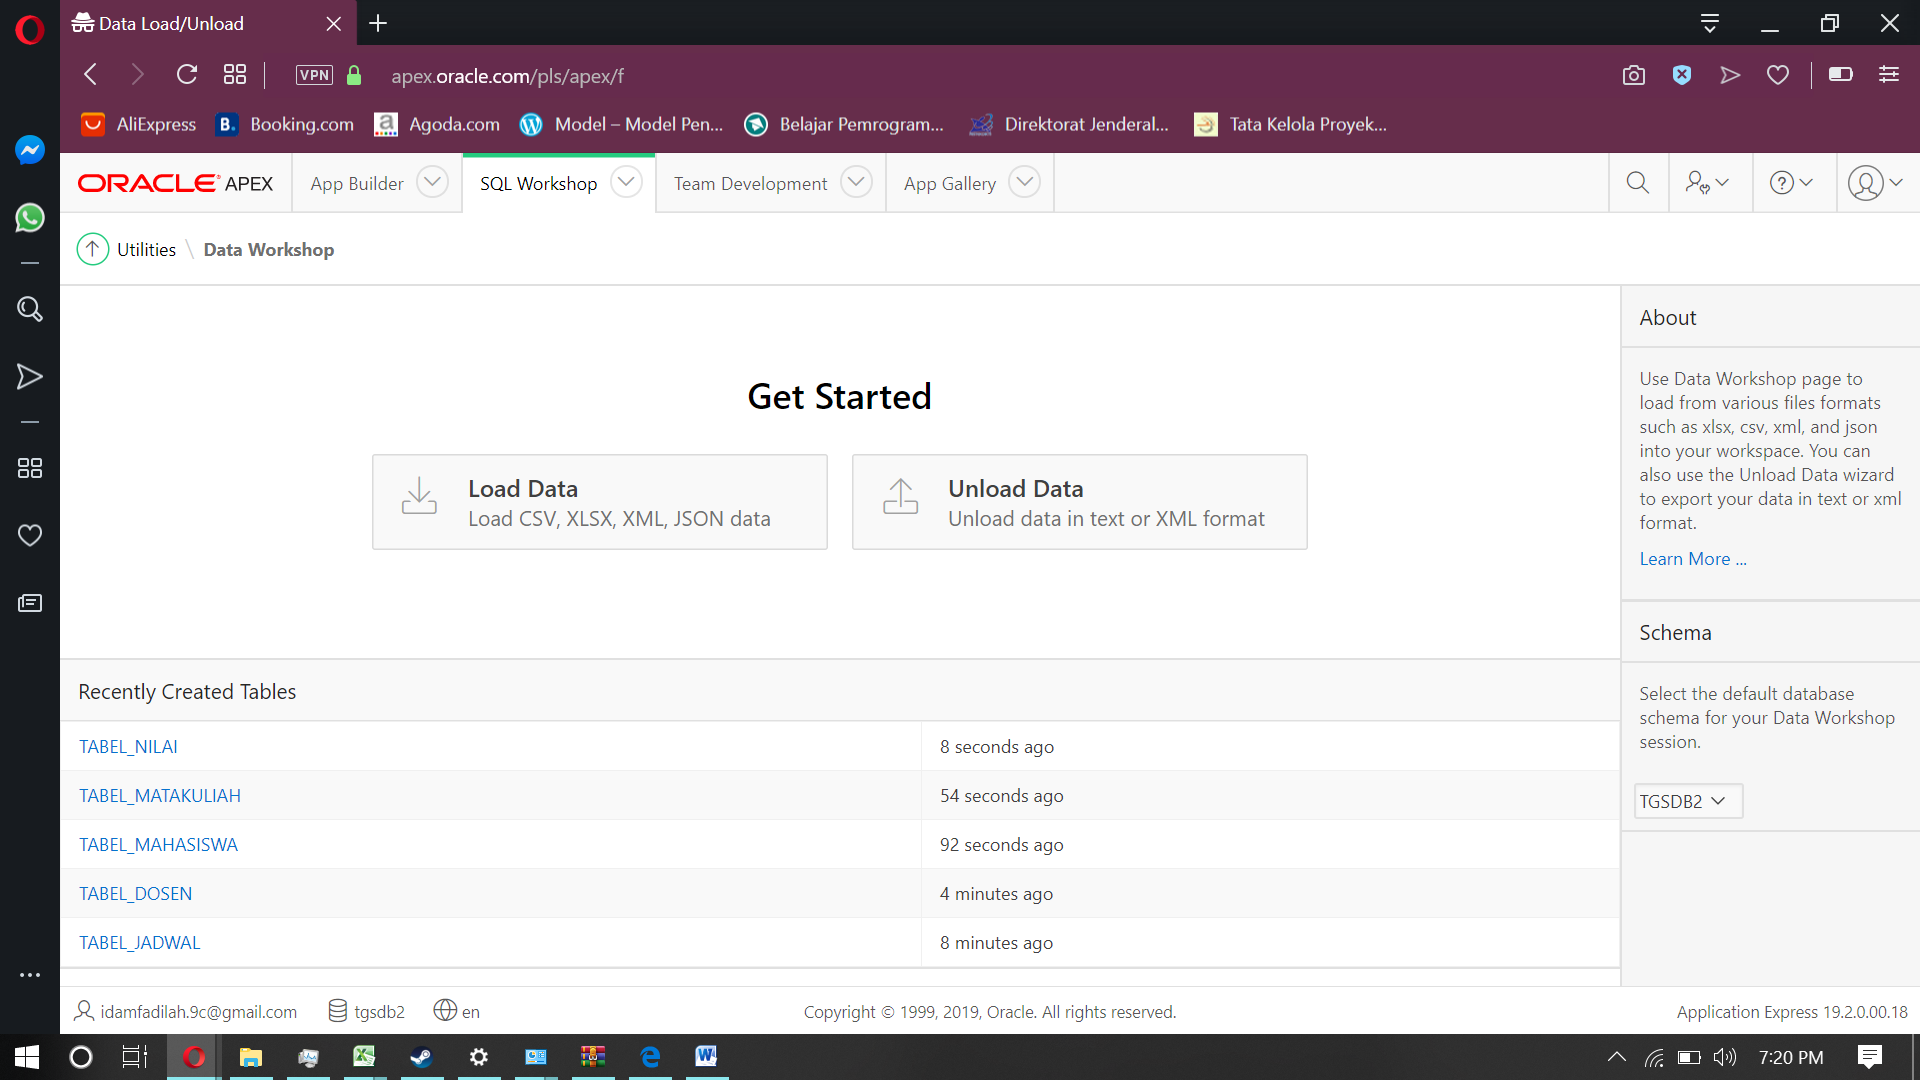
\includegraphics[width=10cm]{excel to db tabel/Screenshot (147).png}\\
	\end{itemize}
\section*{cara membuat aplikasi websheet}
\paragraph{}
\begin{itemize}

	\item jika sudah menambahkan tabel yang diperlukan maka masuk ketahap pembuatan aplikasi, pertama klik app builder/websheet applications\\
	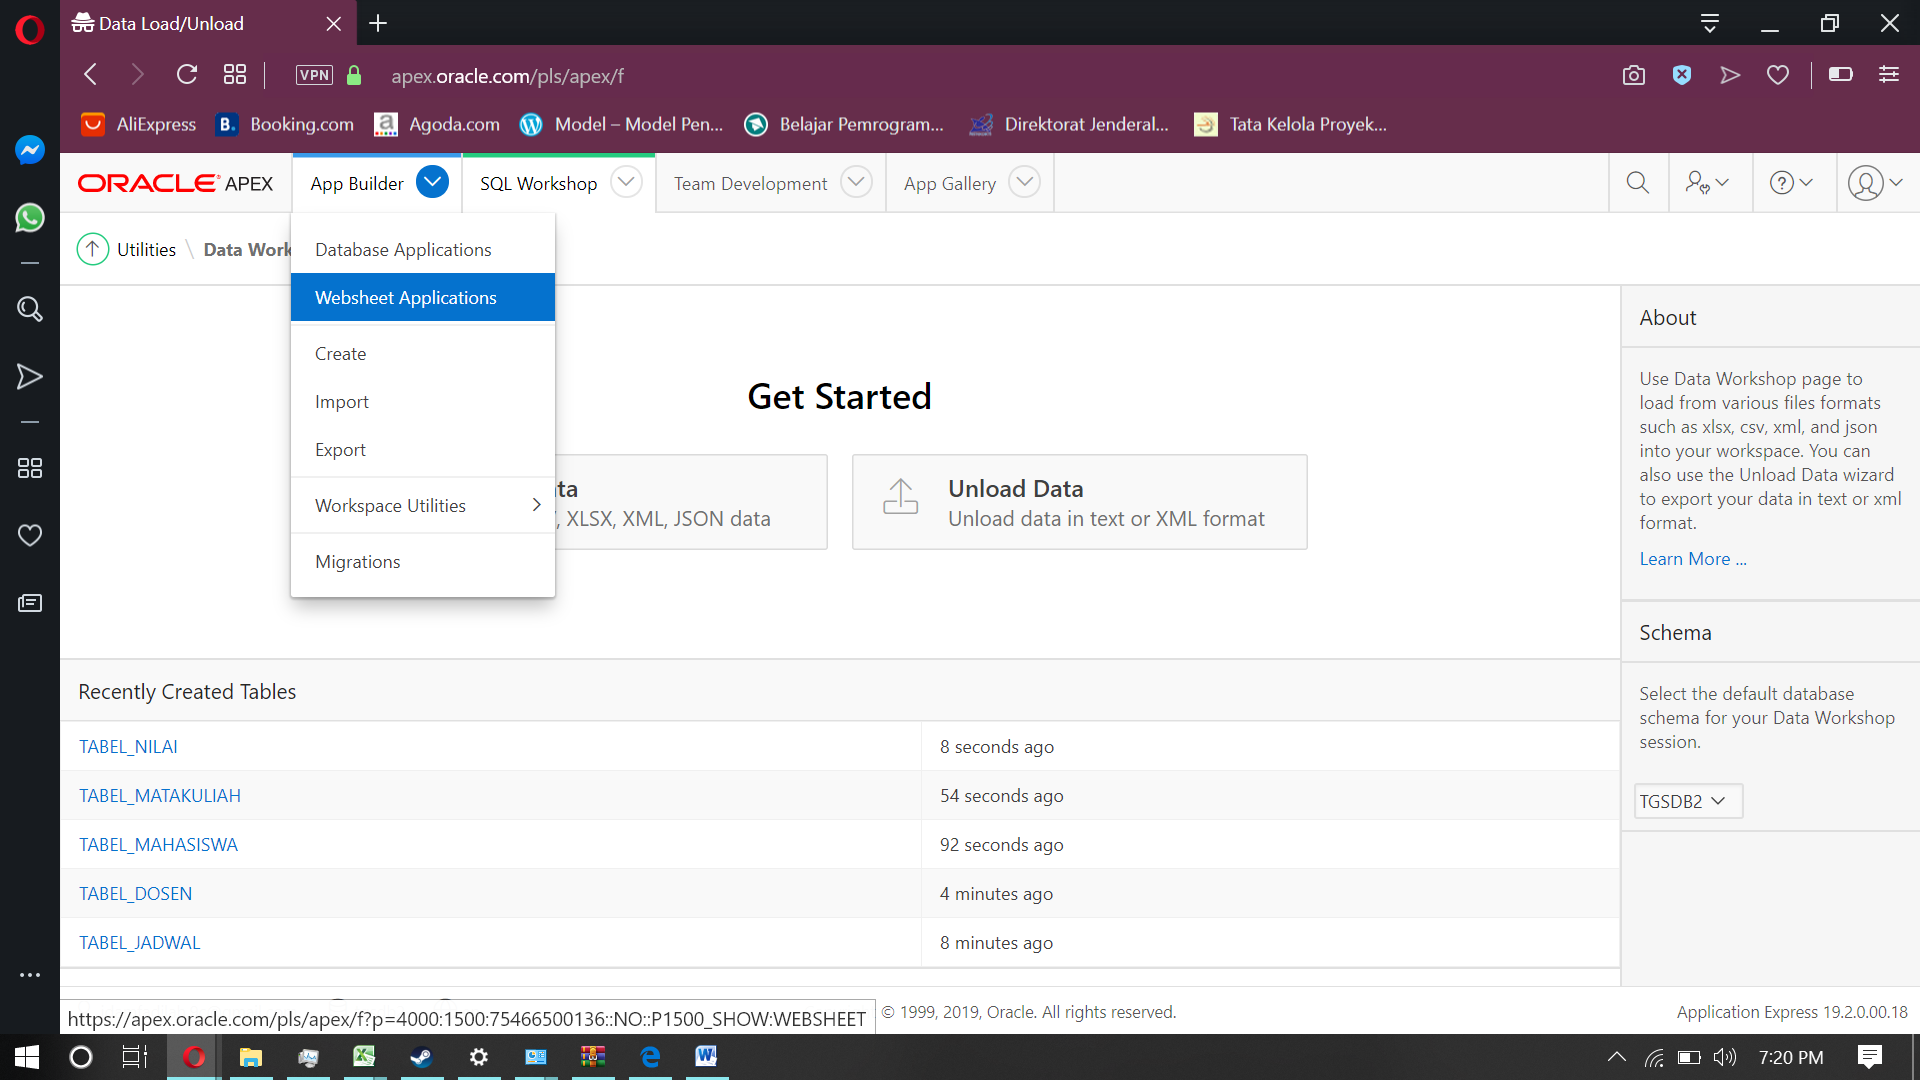
\includegraphics[width=10cm]{aplikasi websheet/Screenshot (148).png}\\ 
	\item klik "Create a New App"\\
	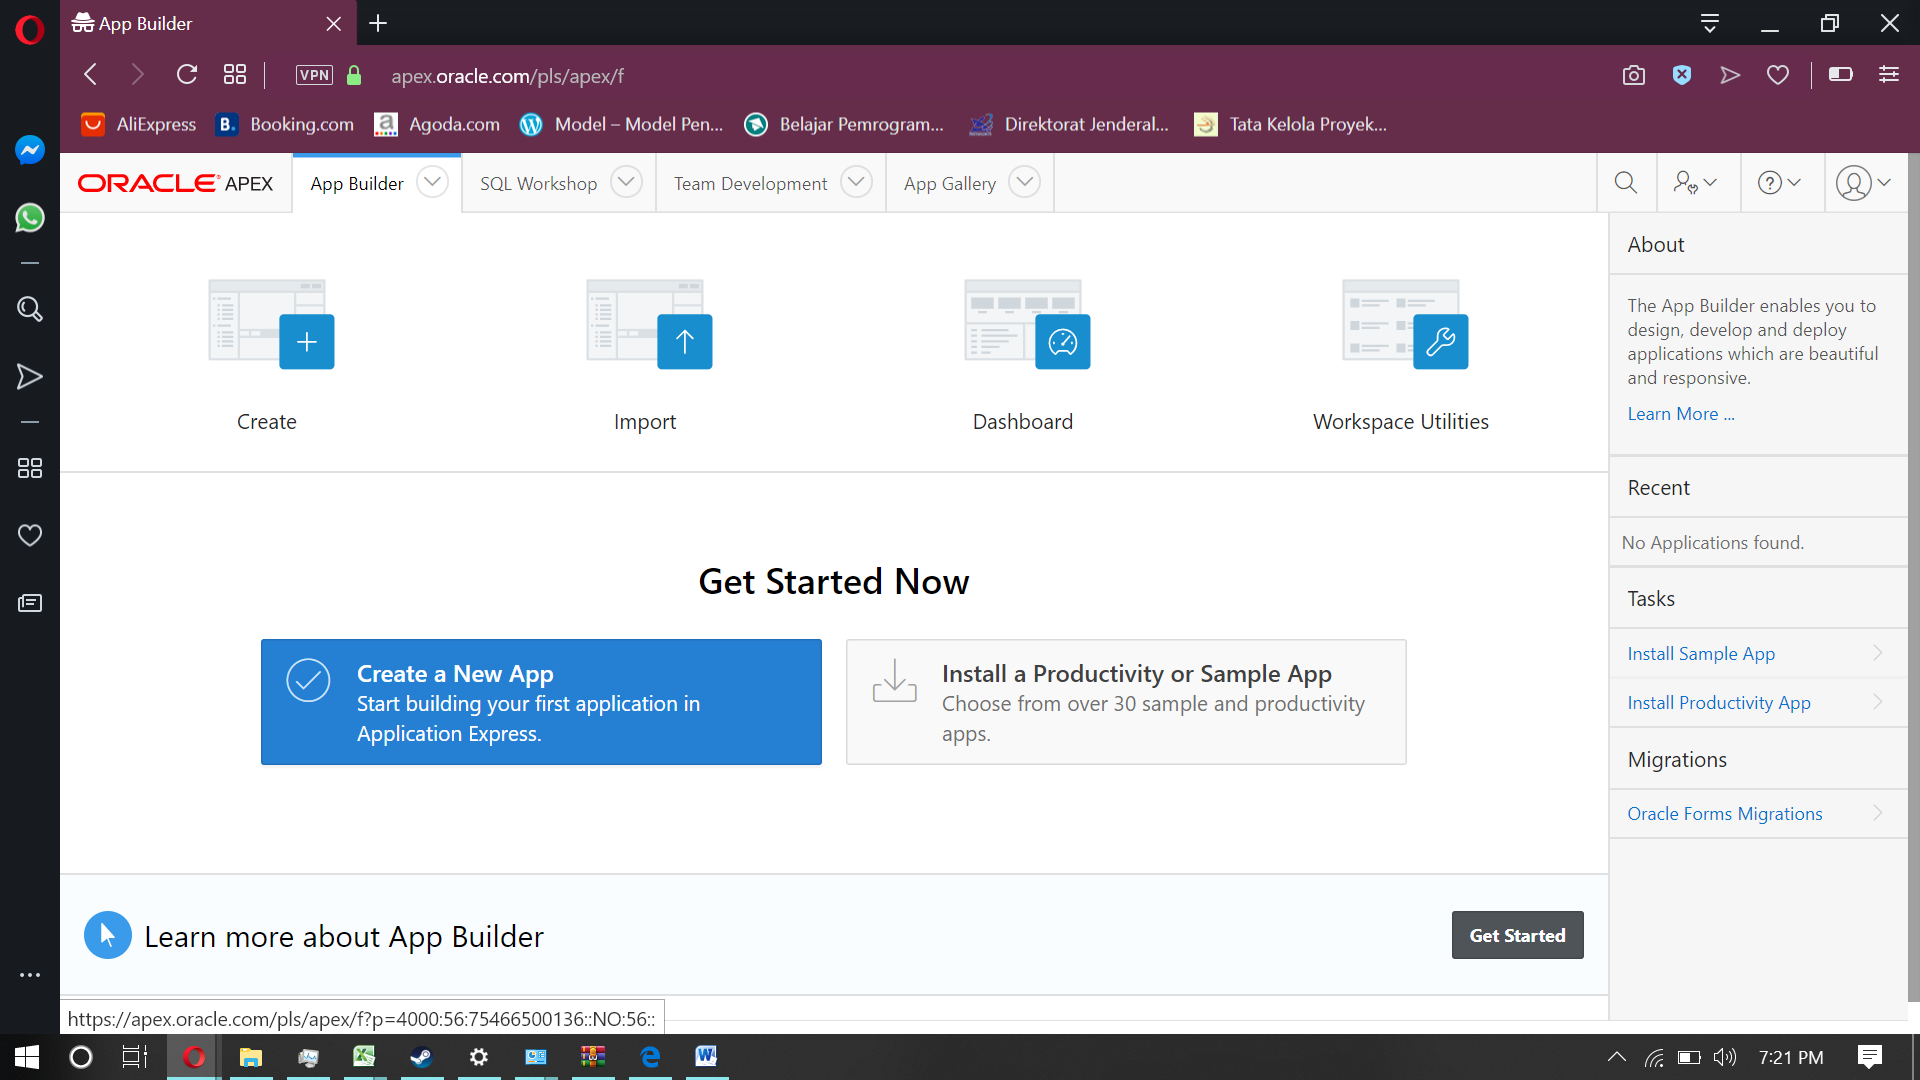
\includegraphics[width=10cm]{aplikasi websheet/Screenshot (149).png}\\ 
	\item klik "new application"\\
	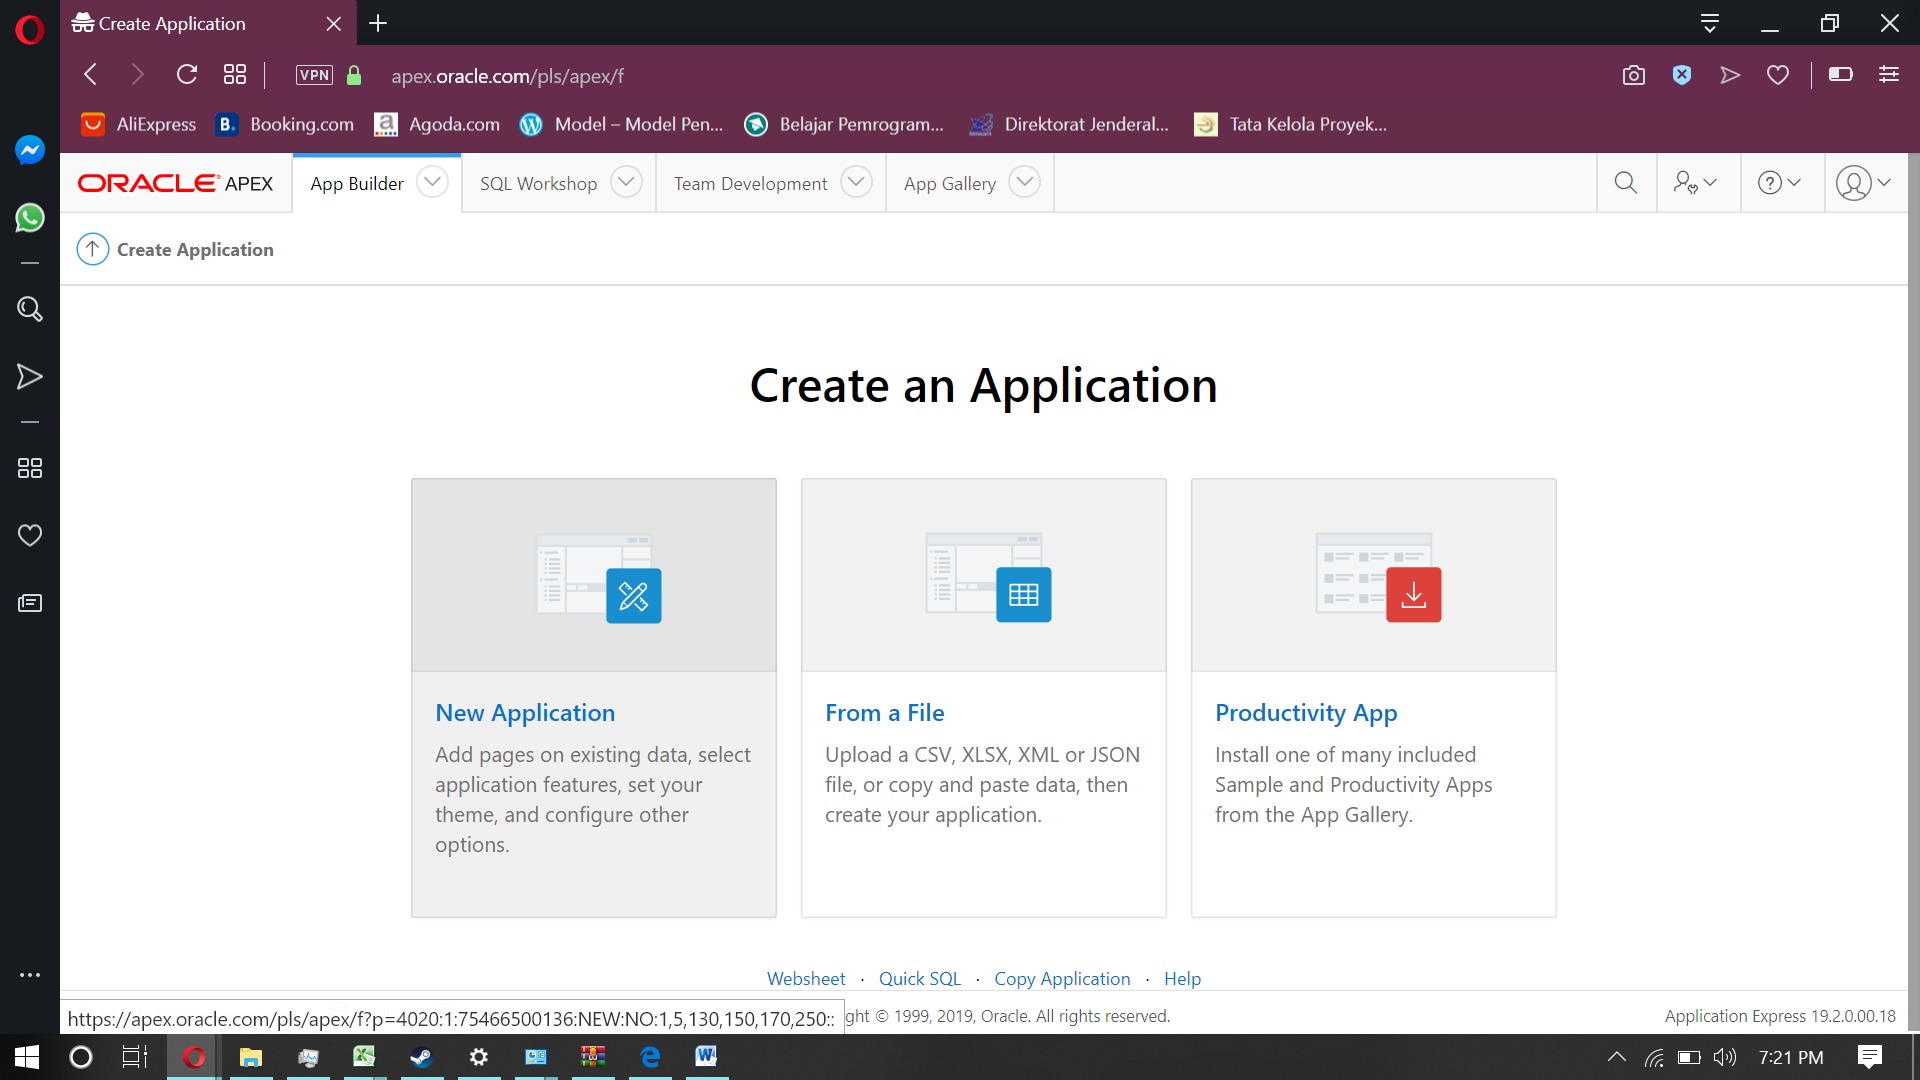
\includegraphics[width=10cm]{aplikasi websheet/Screenshot (150).png}\\ 
	\item isi nama aplikasi, lalu tambahkan page dengan klik "add page"\\
	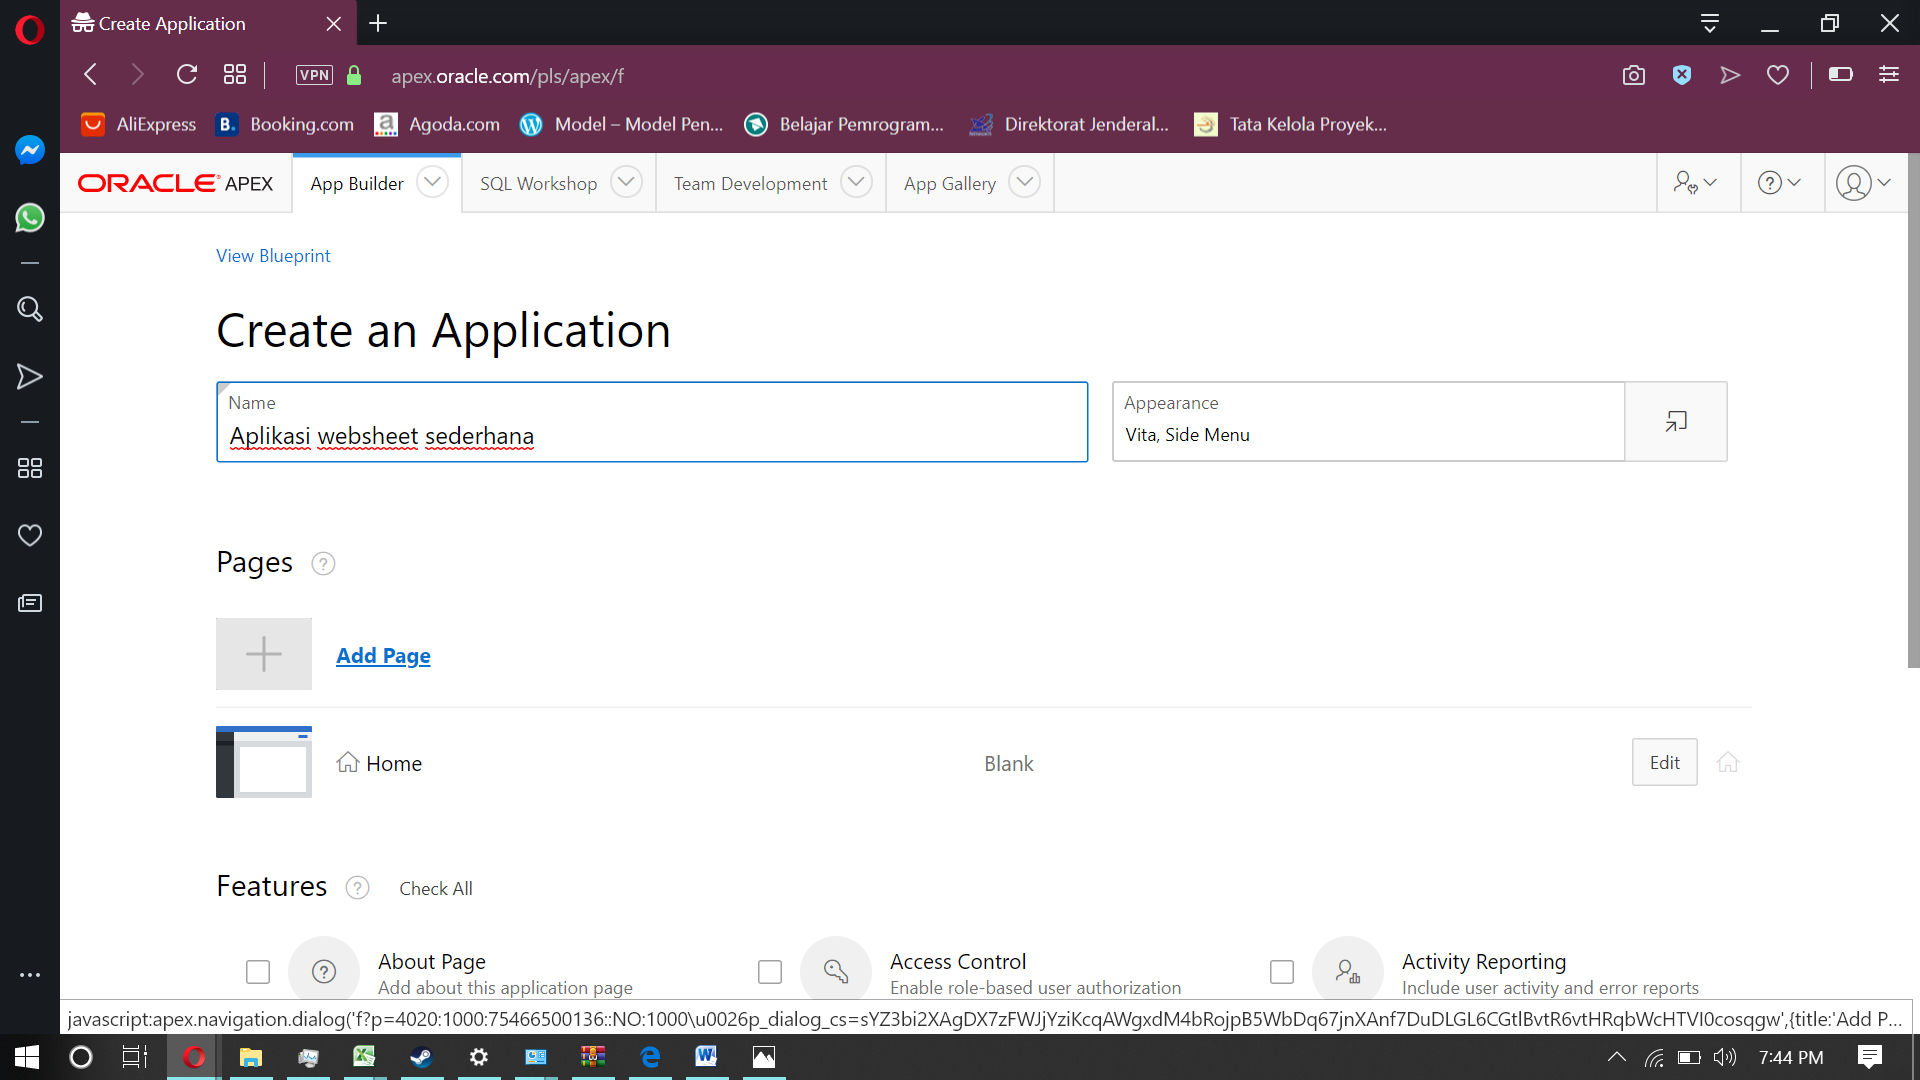
\includegraphics[width=10cm]{aplikasi websheet/Screenshot (155).png}\\ 
	\item disini sudah disediakan berbagai macam page yang bisa dipilih, untuk sekarang kita akan coba membuat page "interactive report"\\
	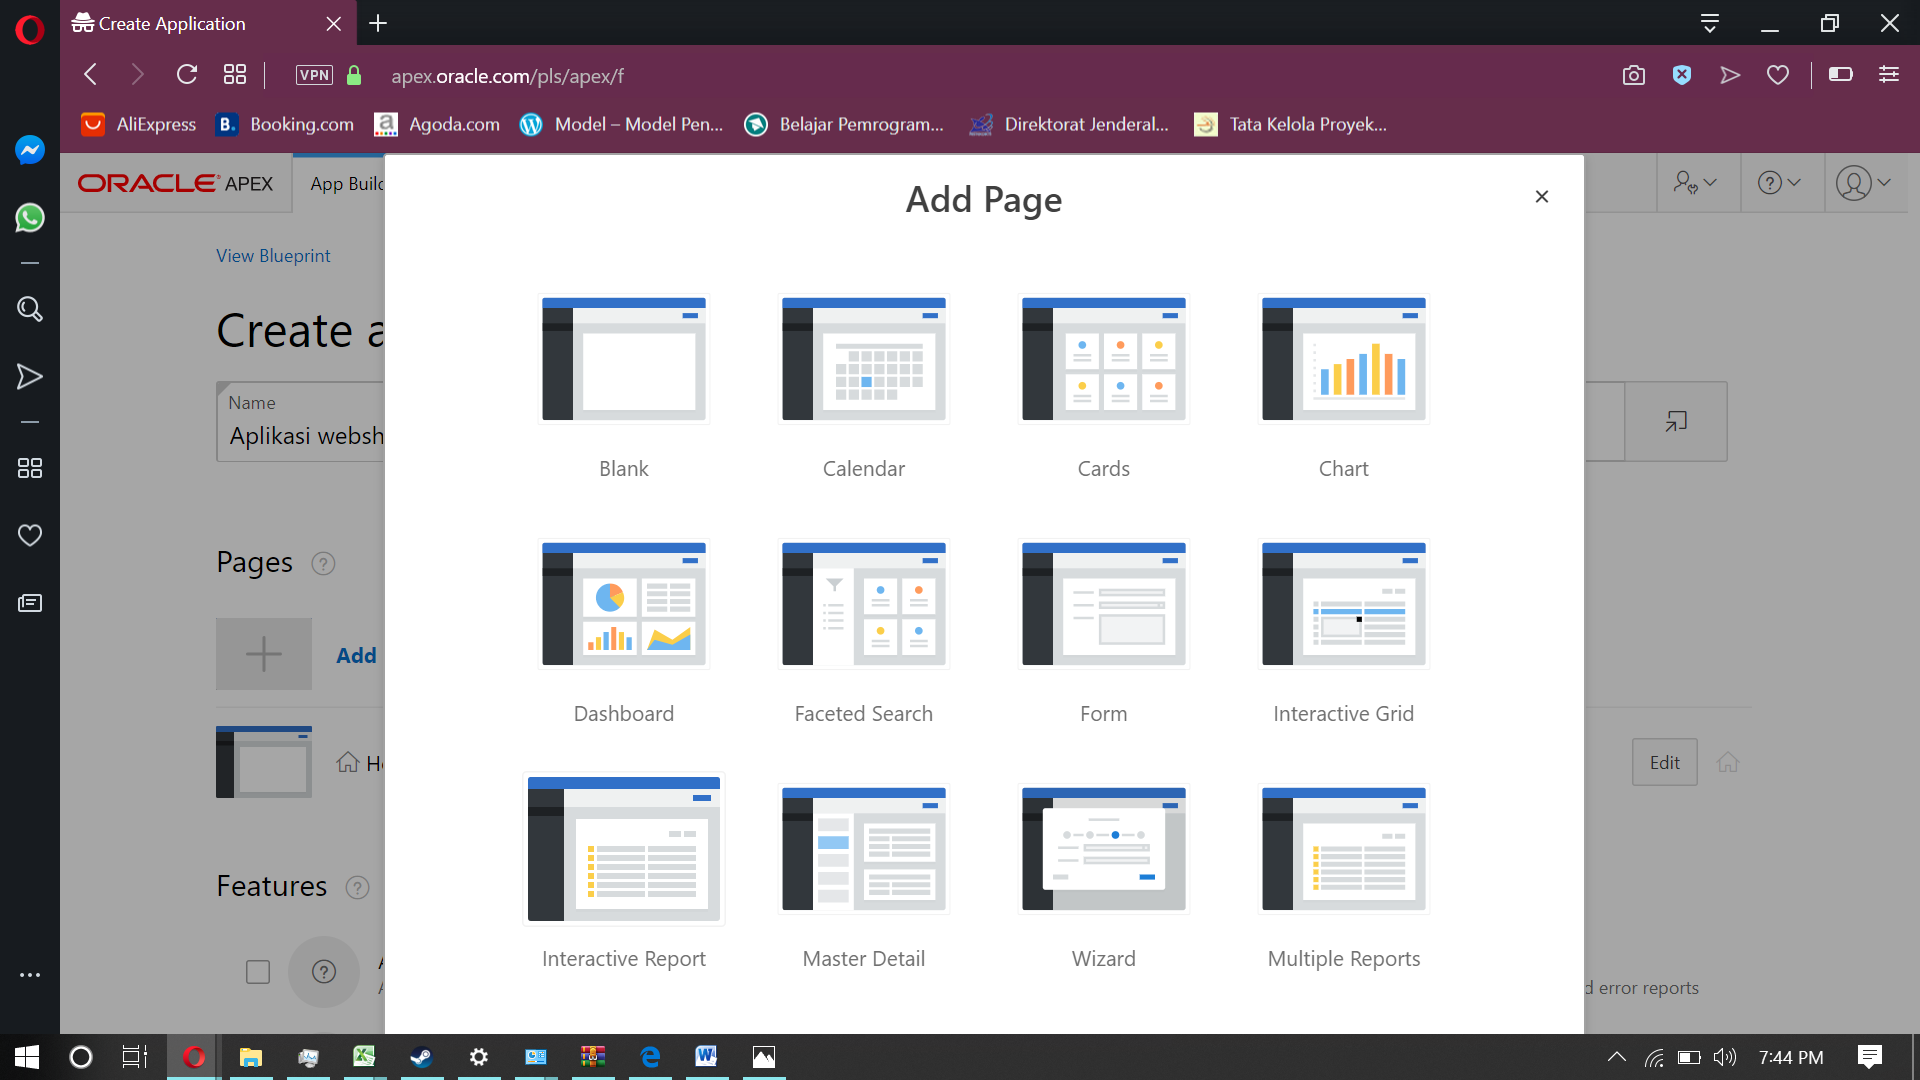
\includegraphics[width=10cm]{aplikasi websheet/Screenshot (156).png}\\ 
	\item isi page name lalu klik menu bar pada "table or view" sebelah kanan\\
	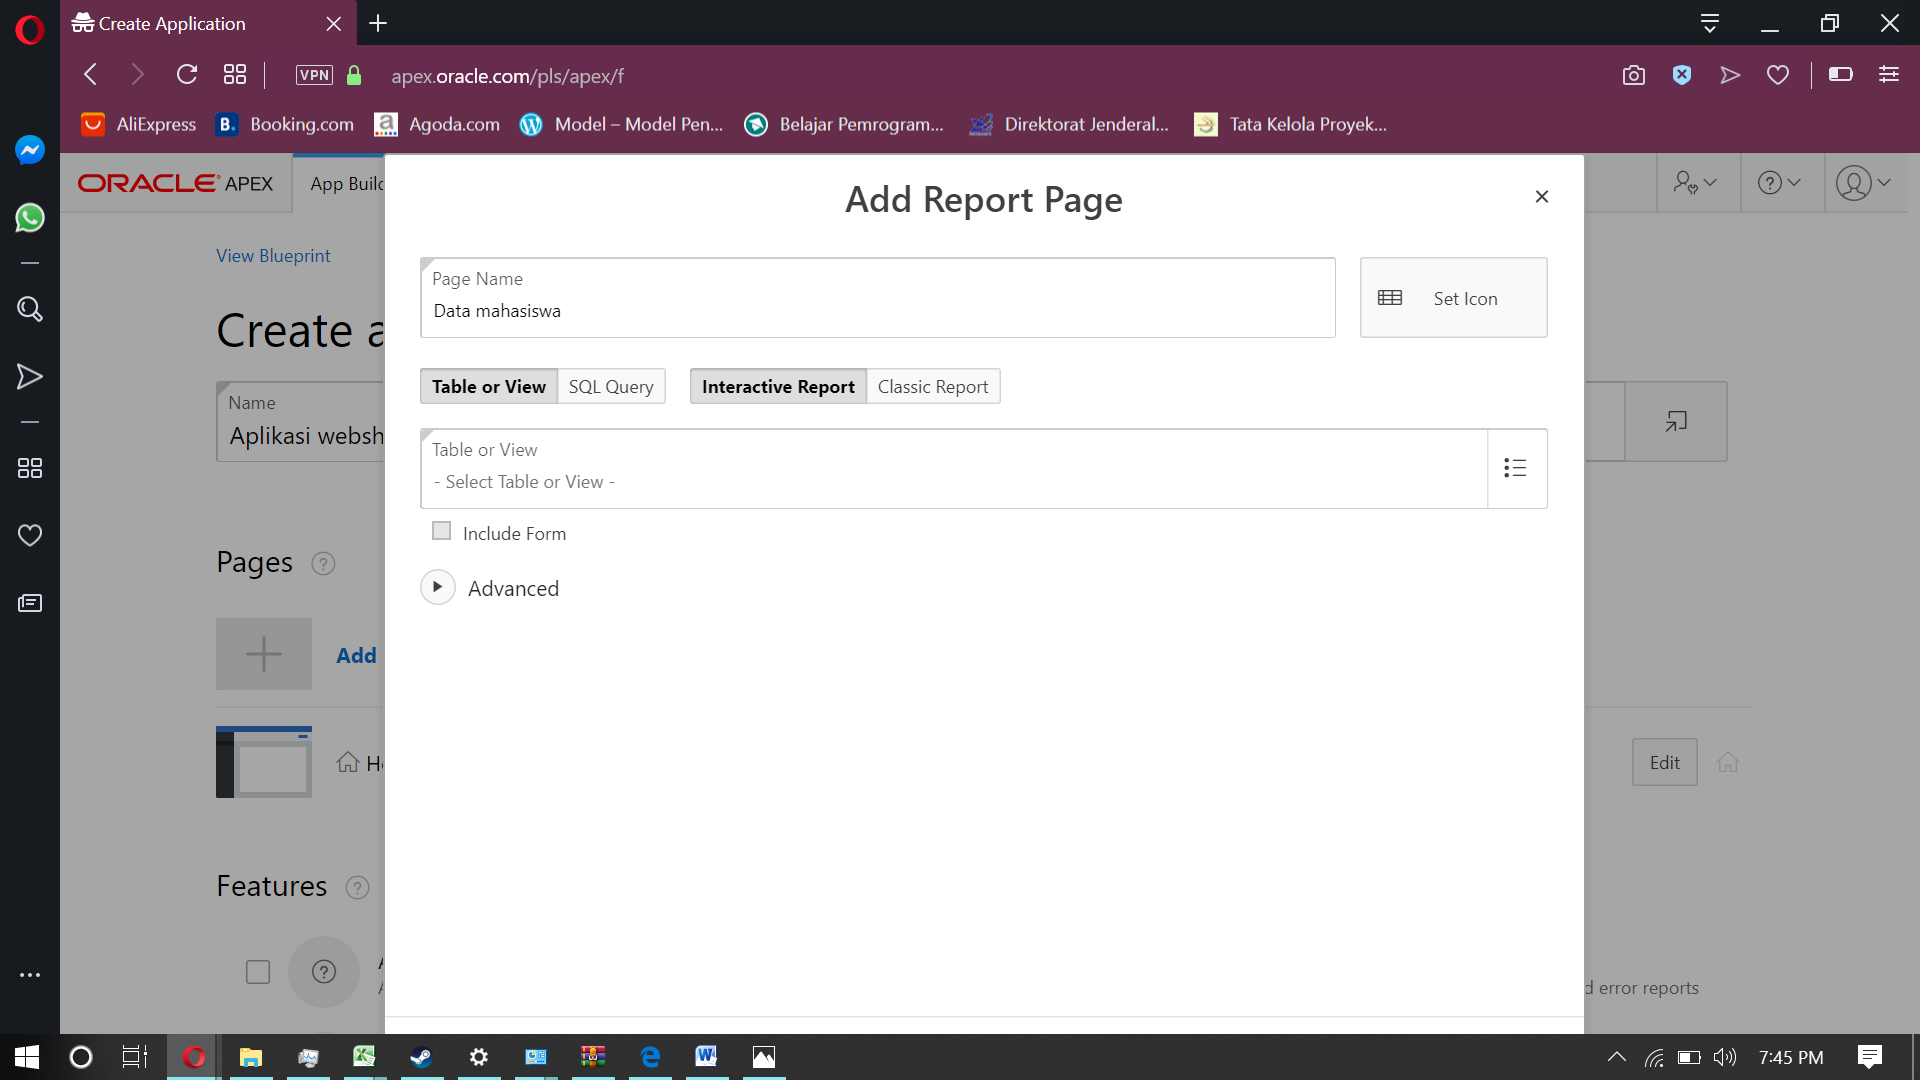
\includegraphics[width=10cm]{aplikasi websheet/Screenshot (157).png}\\ 
	\item pilih tabel yang akan ditampilkan\\
	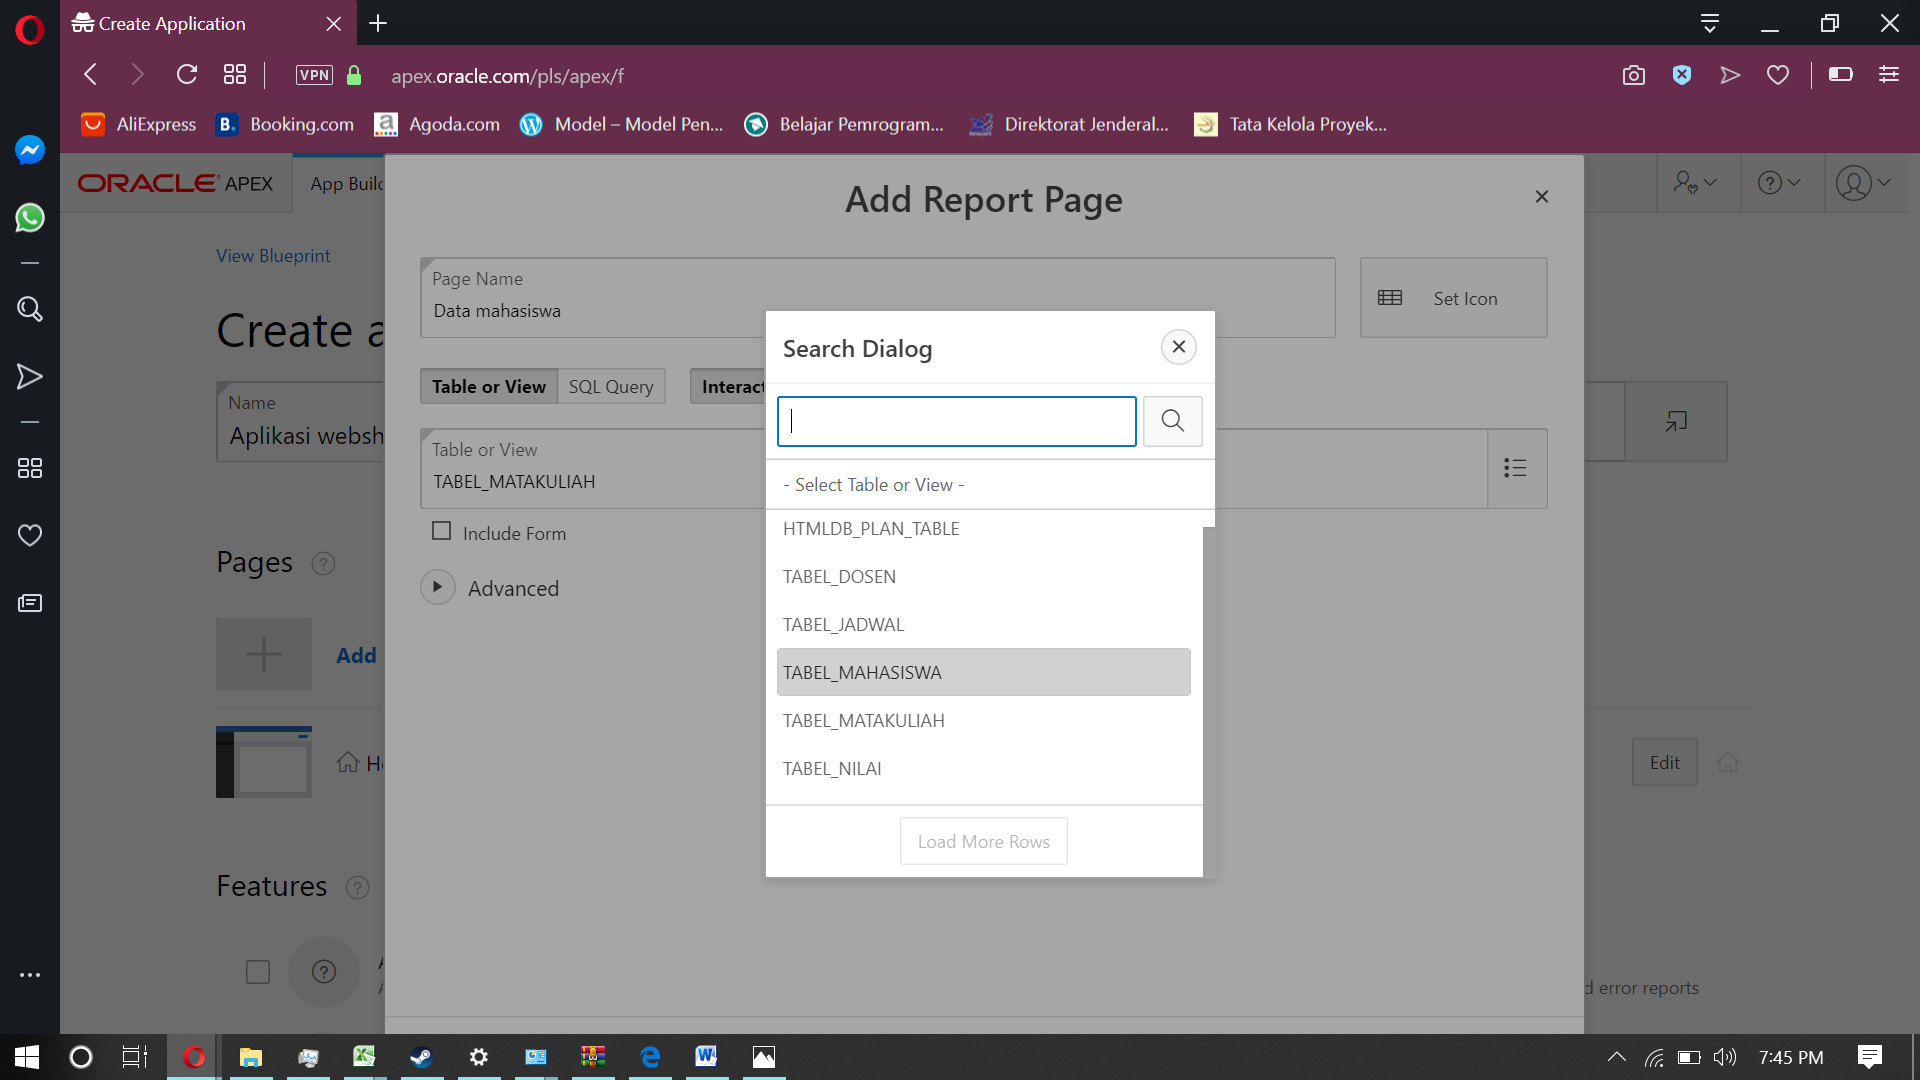
\includegraphics[width=10cm]{aplikasi websheet/Screenshot (159).png}\\ 
	\item jika semua telah di isi maka klik "add page"\\
	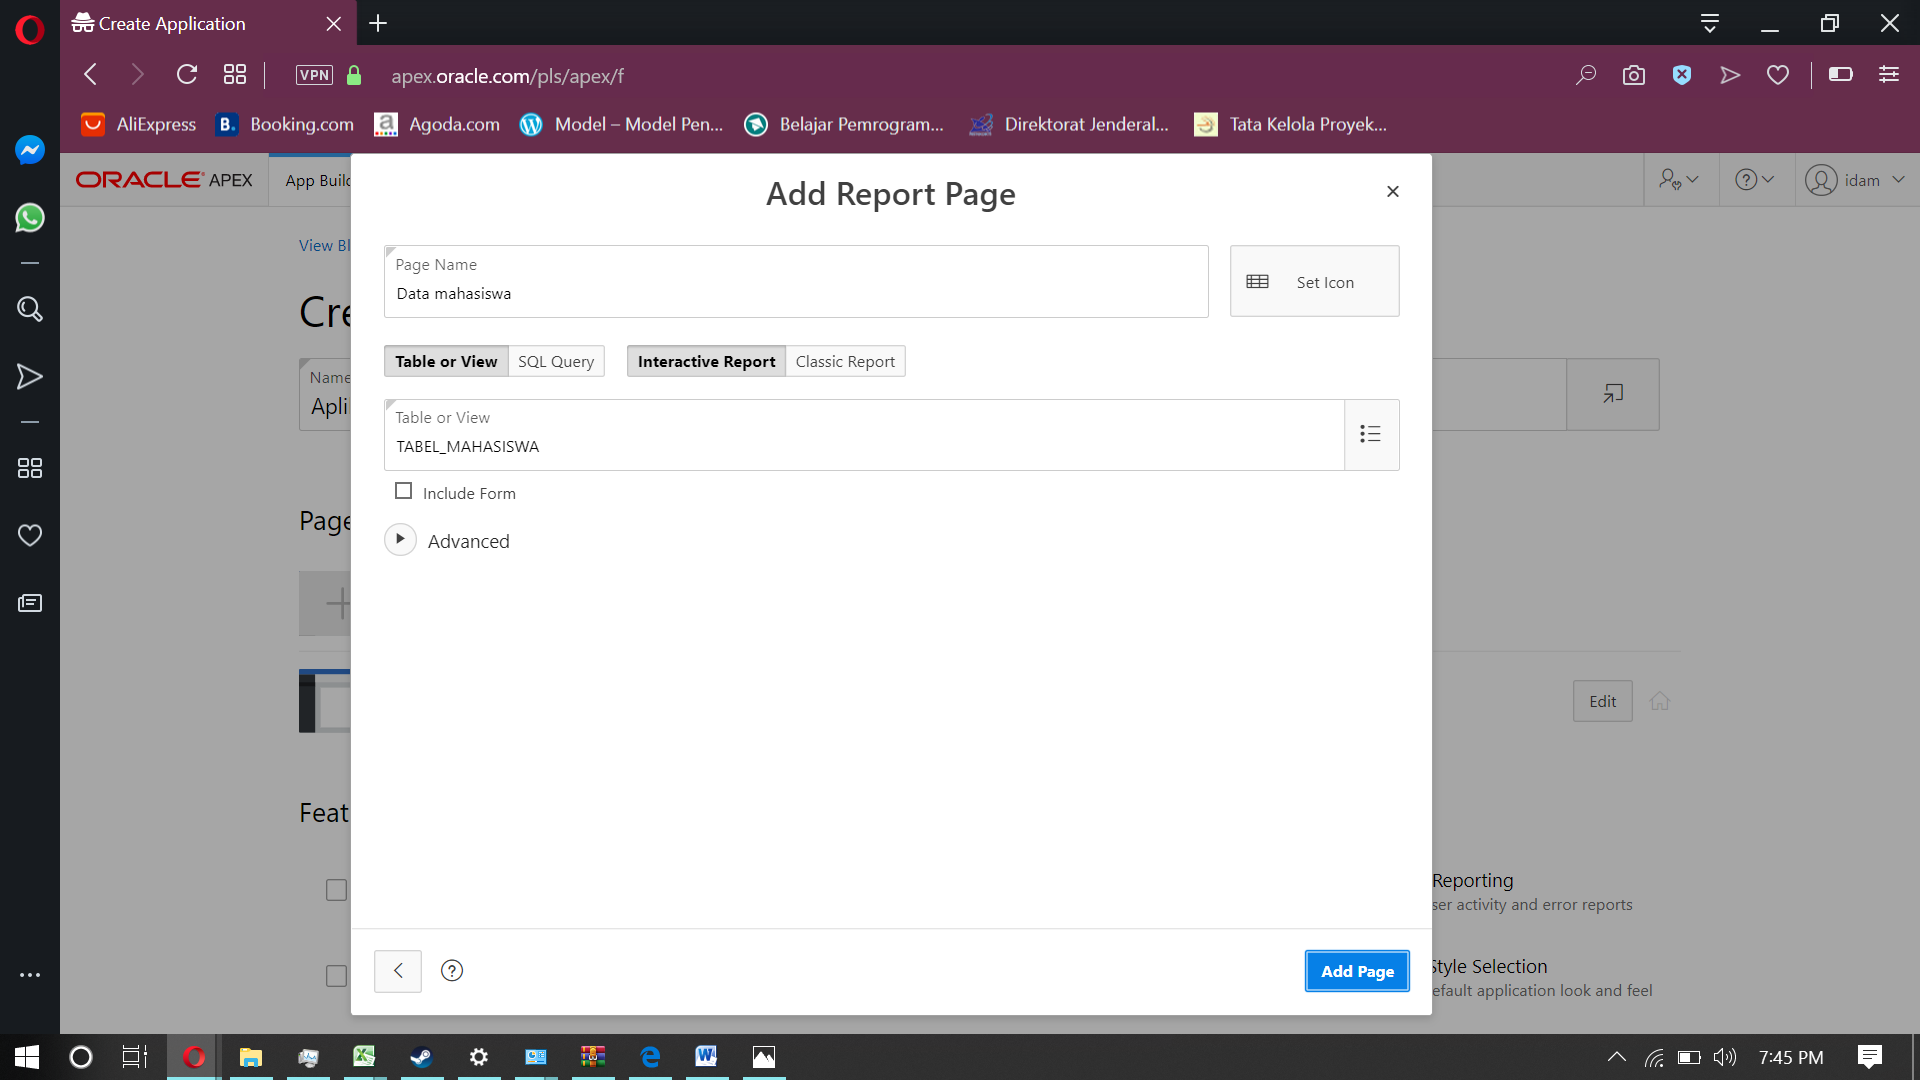
\includegraphics[width=10cm]{aplikasi websheet/Screenshot (160).png}\\ 
	\item disini saya membuat 5 page berdasarkan 5 tabel yang saya buat sebelumnya\\
	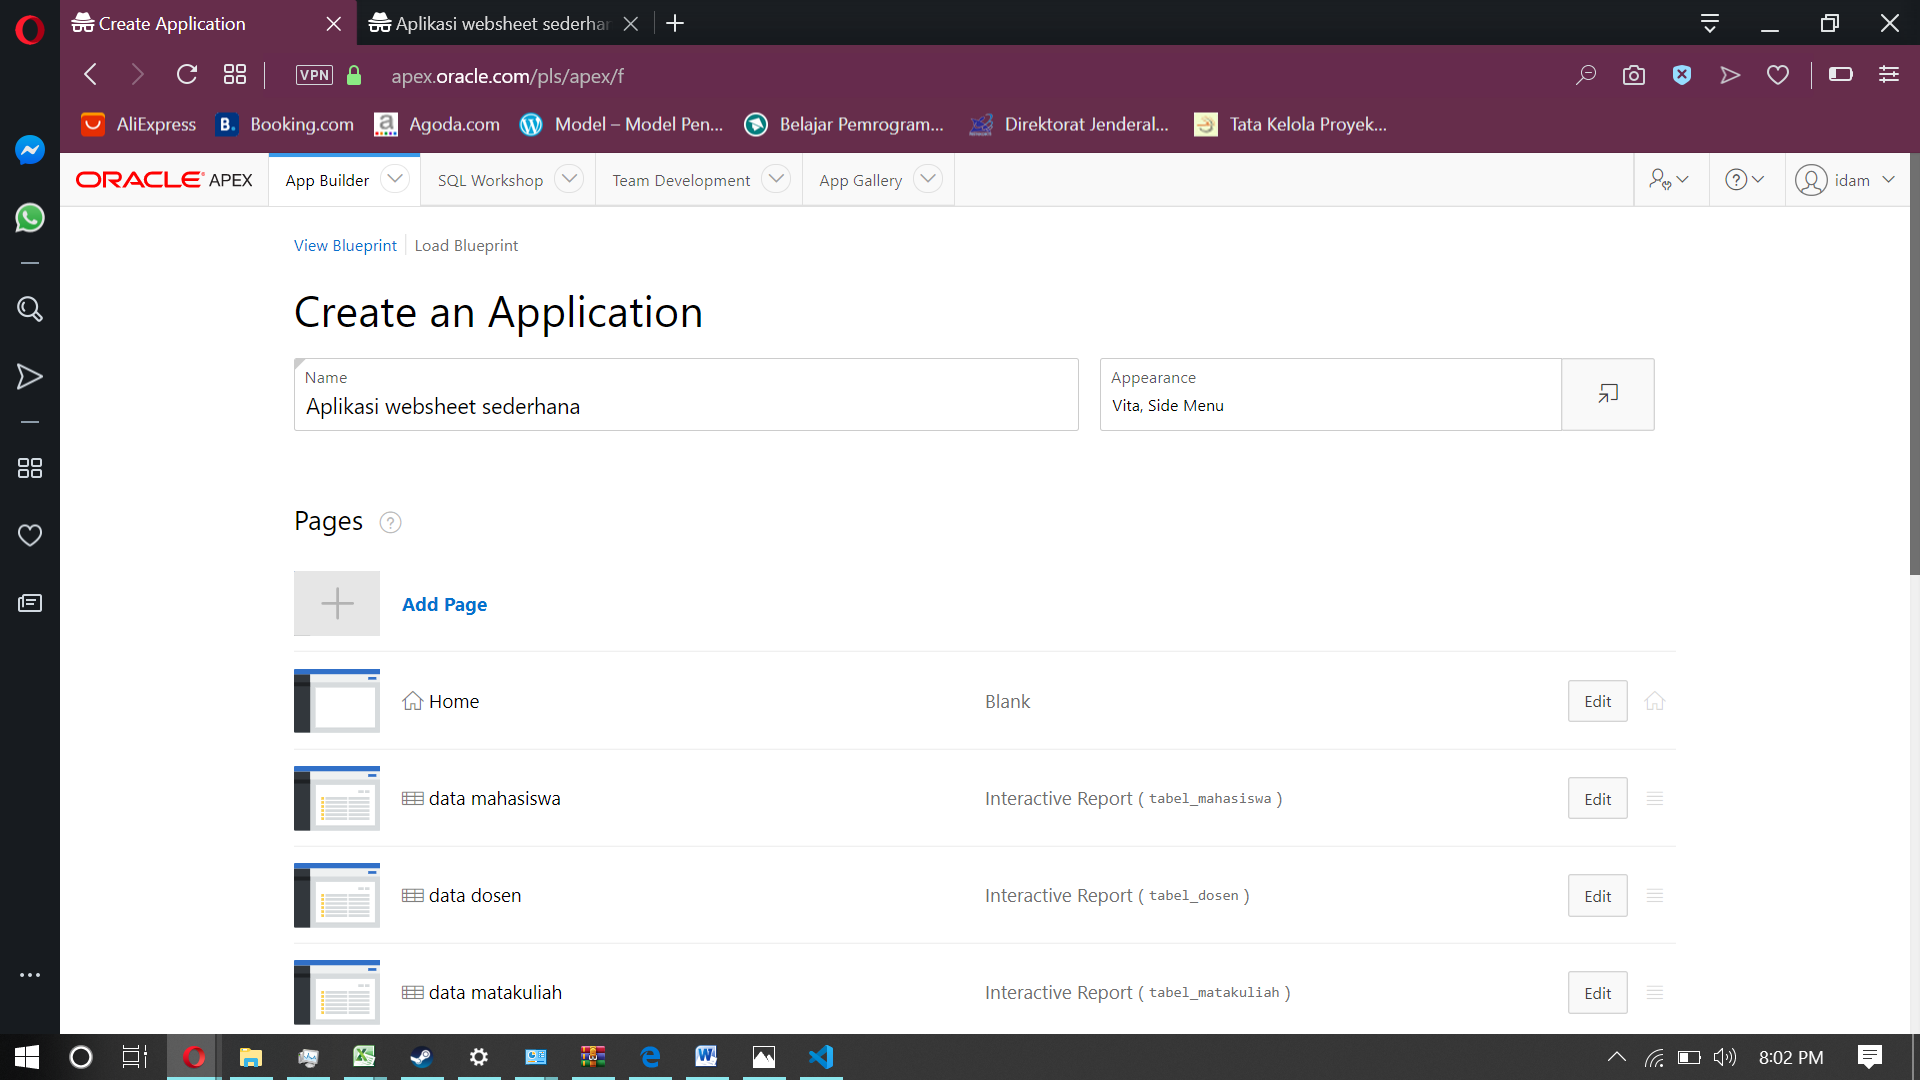
\includegraphics[width=10cm]{aplikasi websheet/Screenshot (161).png}\\ 
	\item jika sudah maka klik "create application"\\
	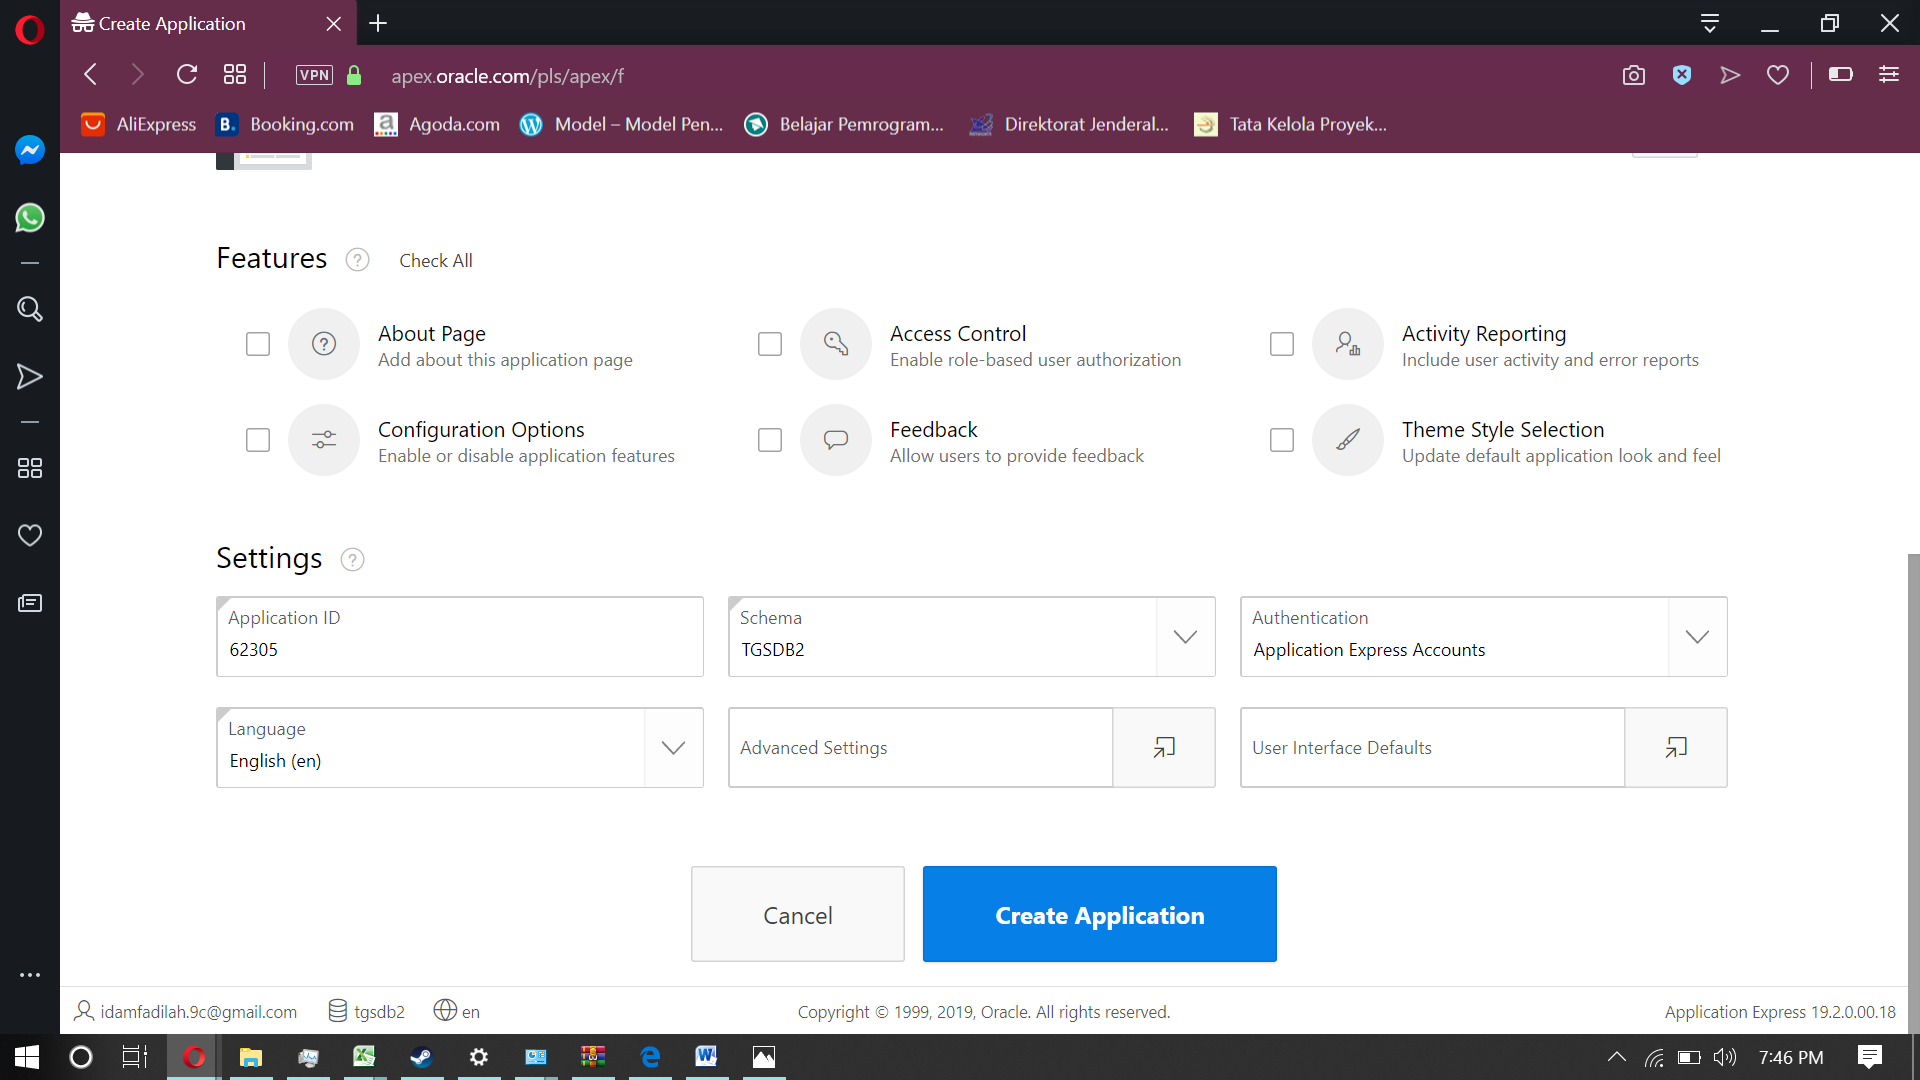
\includegraphics[width=10cm]{aplikasi websheet/Screenshot (162).png}\\ 
	\item jika sudah maka klik "run application"\\
	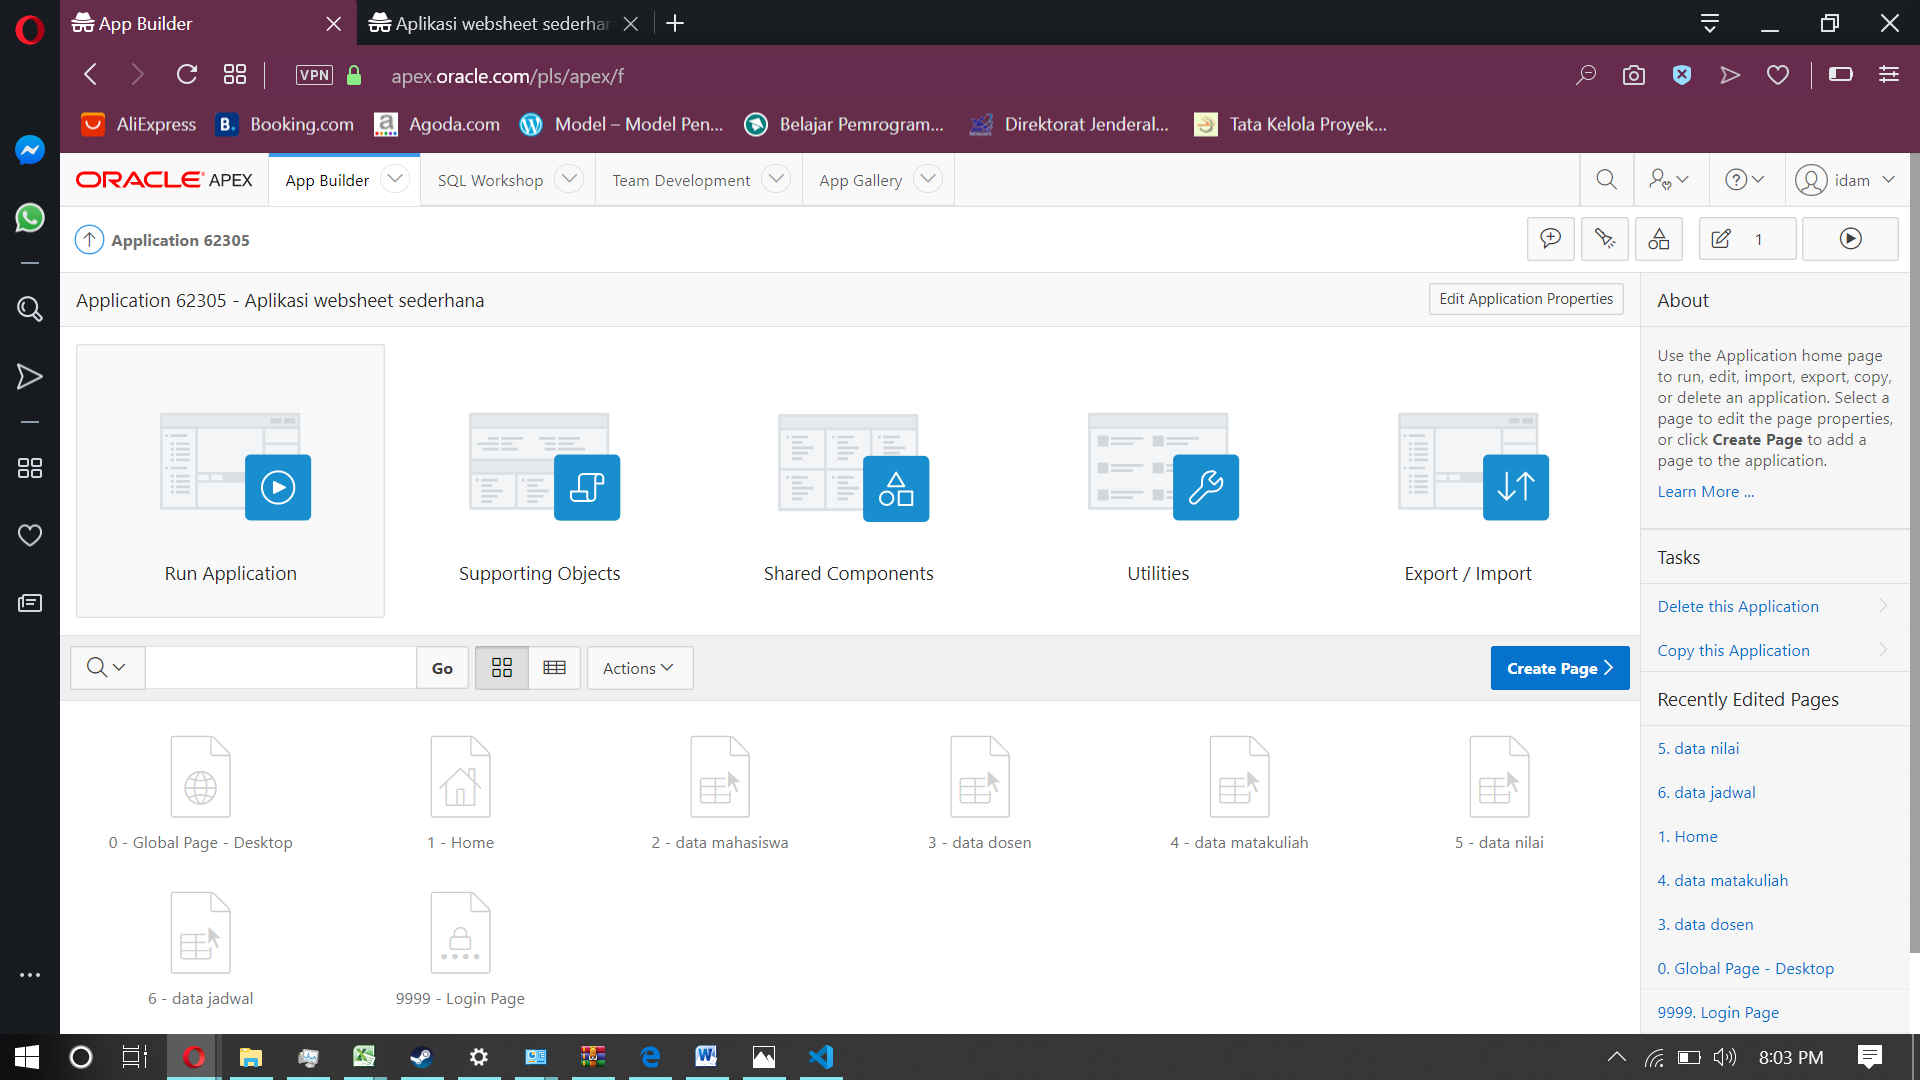
\includegraphics[width=10cm]{aplikasi websheet/Screenshot (163).png}\\ 
	\item isi username dan password yang digunakan pada workspace\\
	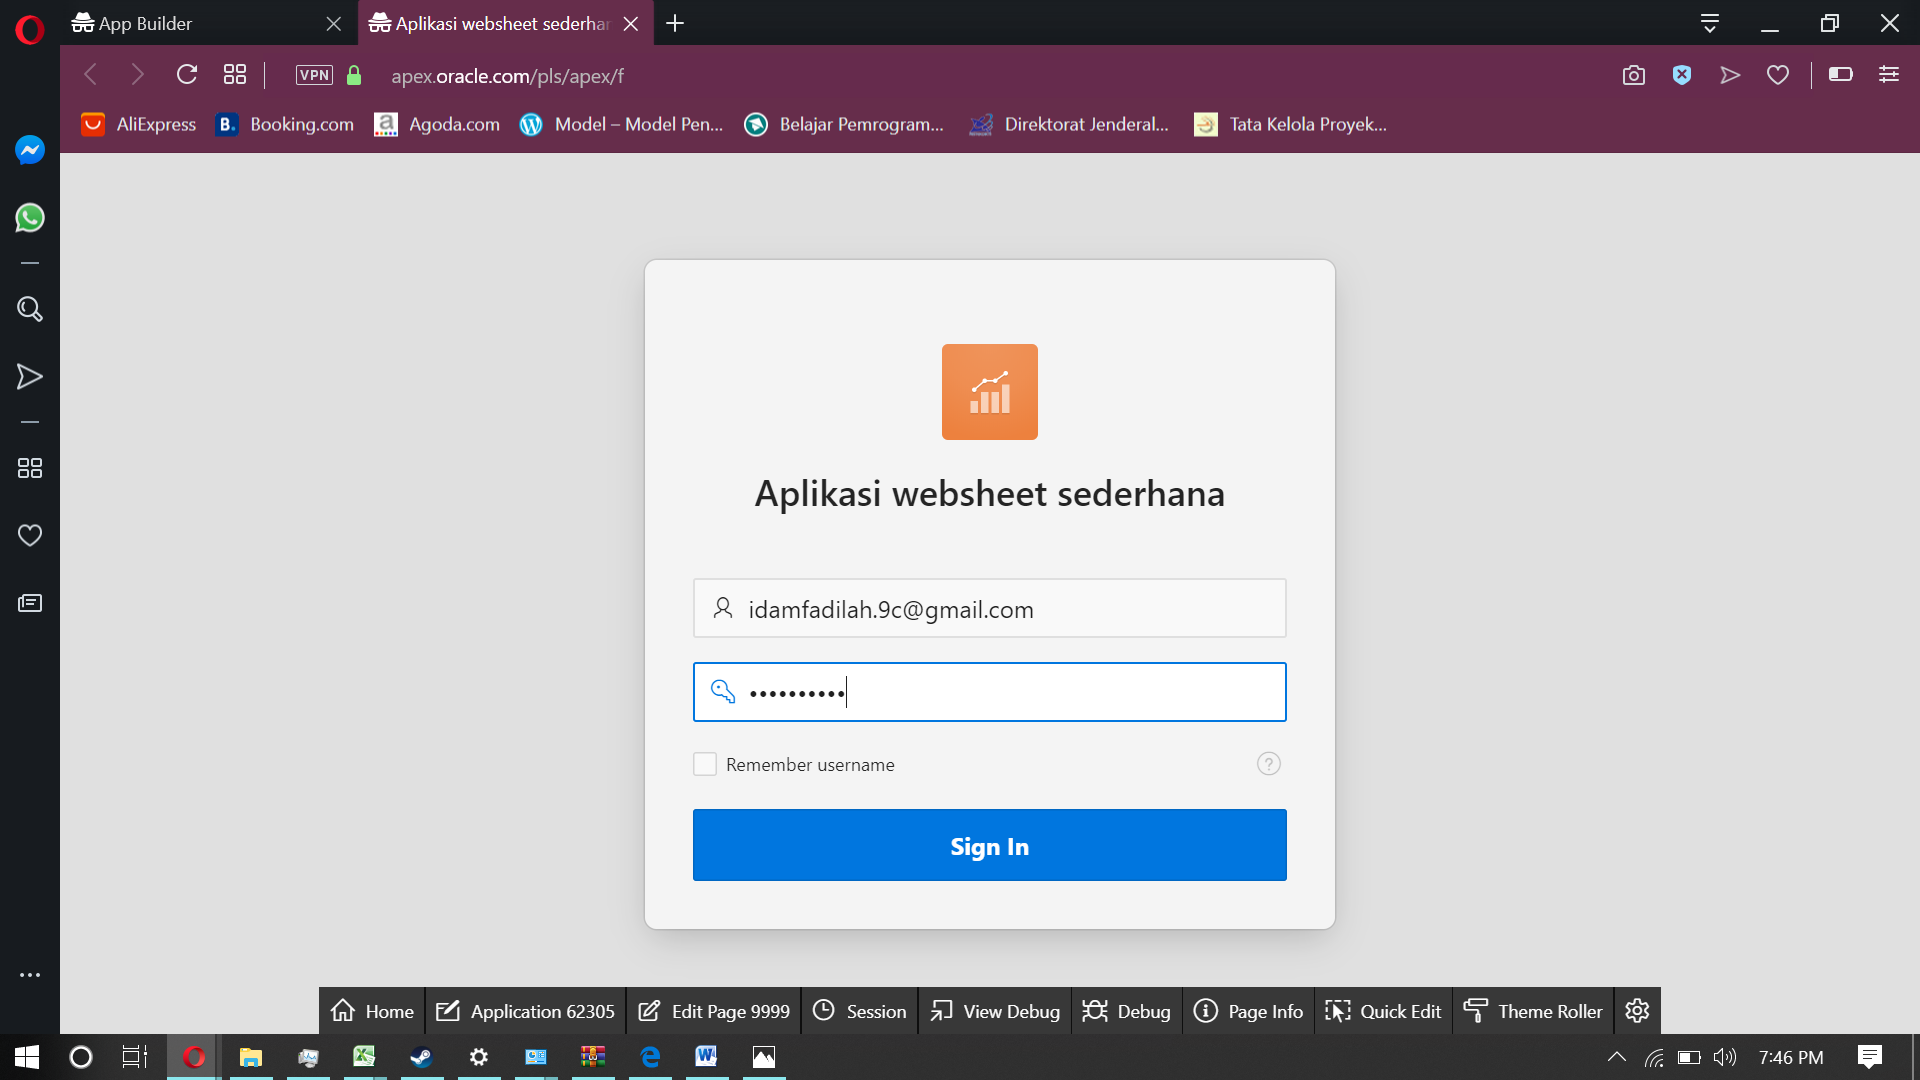
\includegraphics[width=10cm]{aplikasi websheet/Screenshot (164).png}\\ 
	\item maka akan tampil menu home aplikasi yang telah kita buat\\
	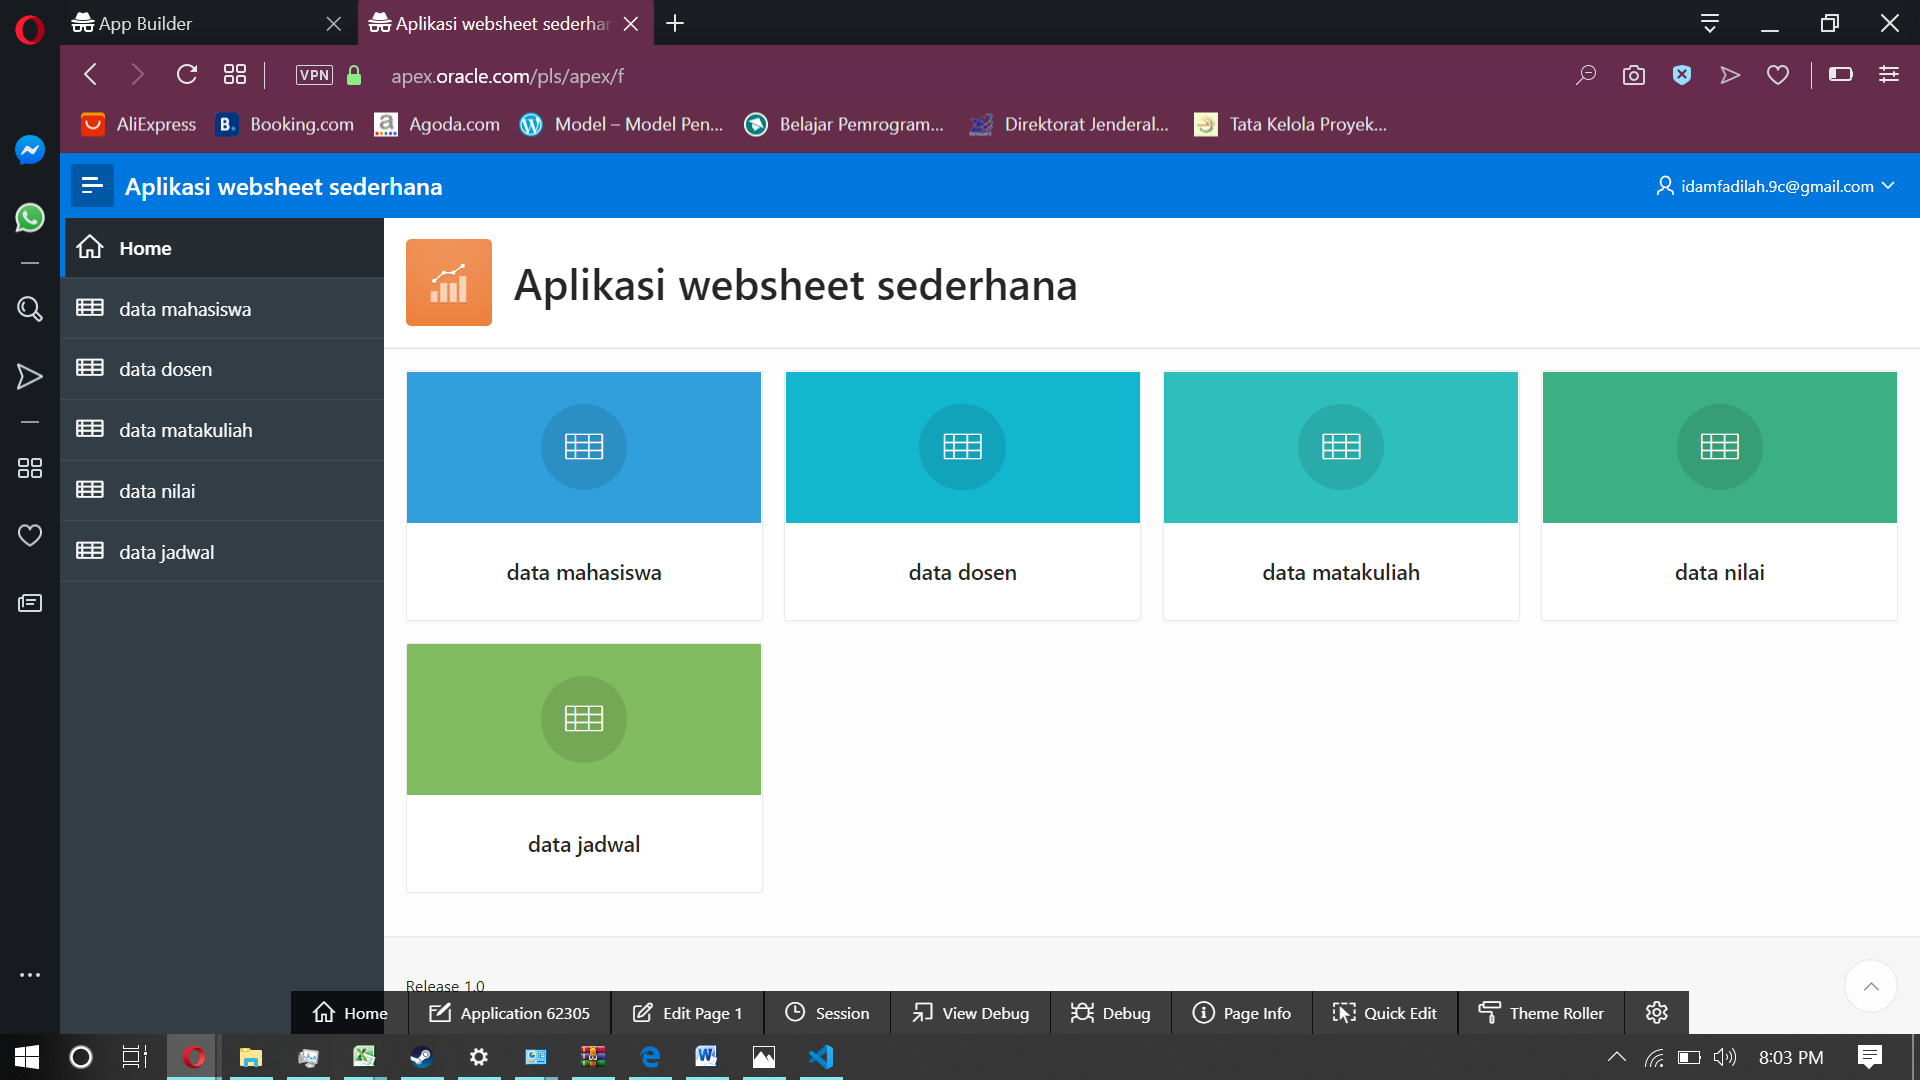
\includegraphics[width=10cm]{aplikasi websheet/Screenshot (169).png}\\ 
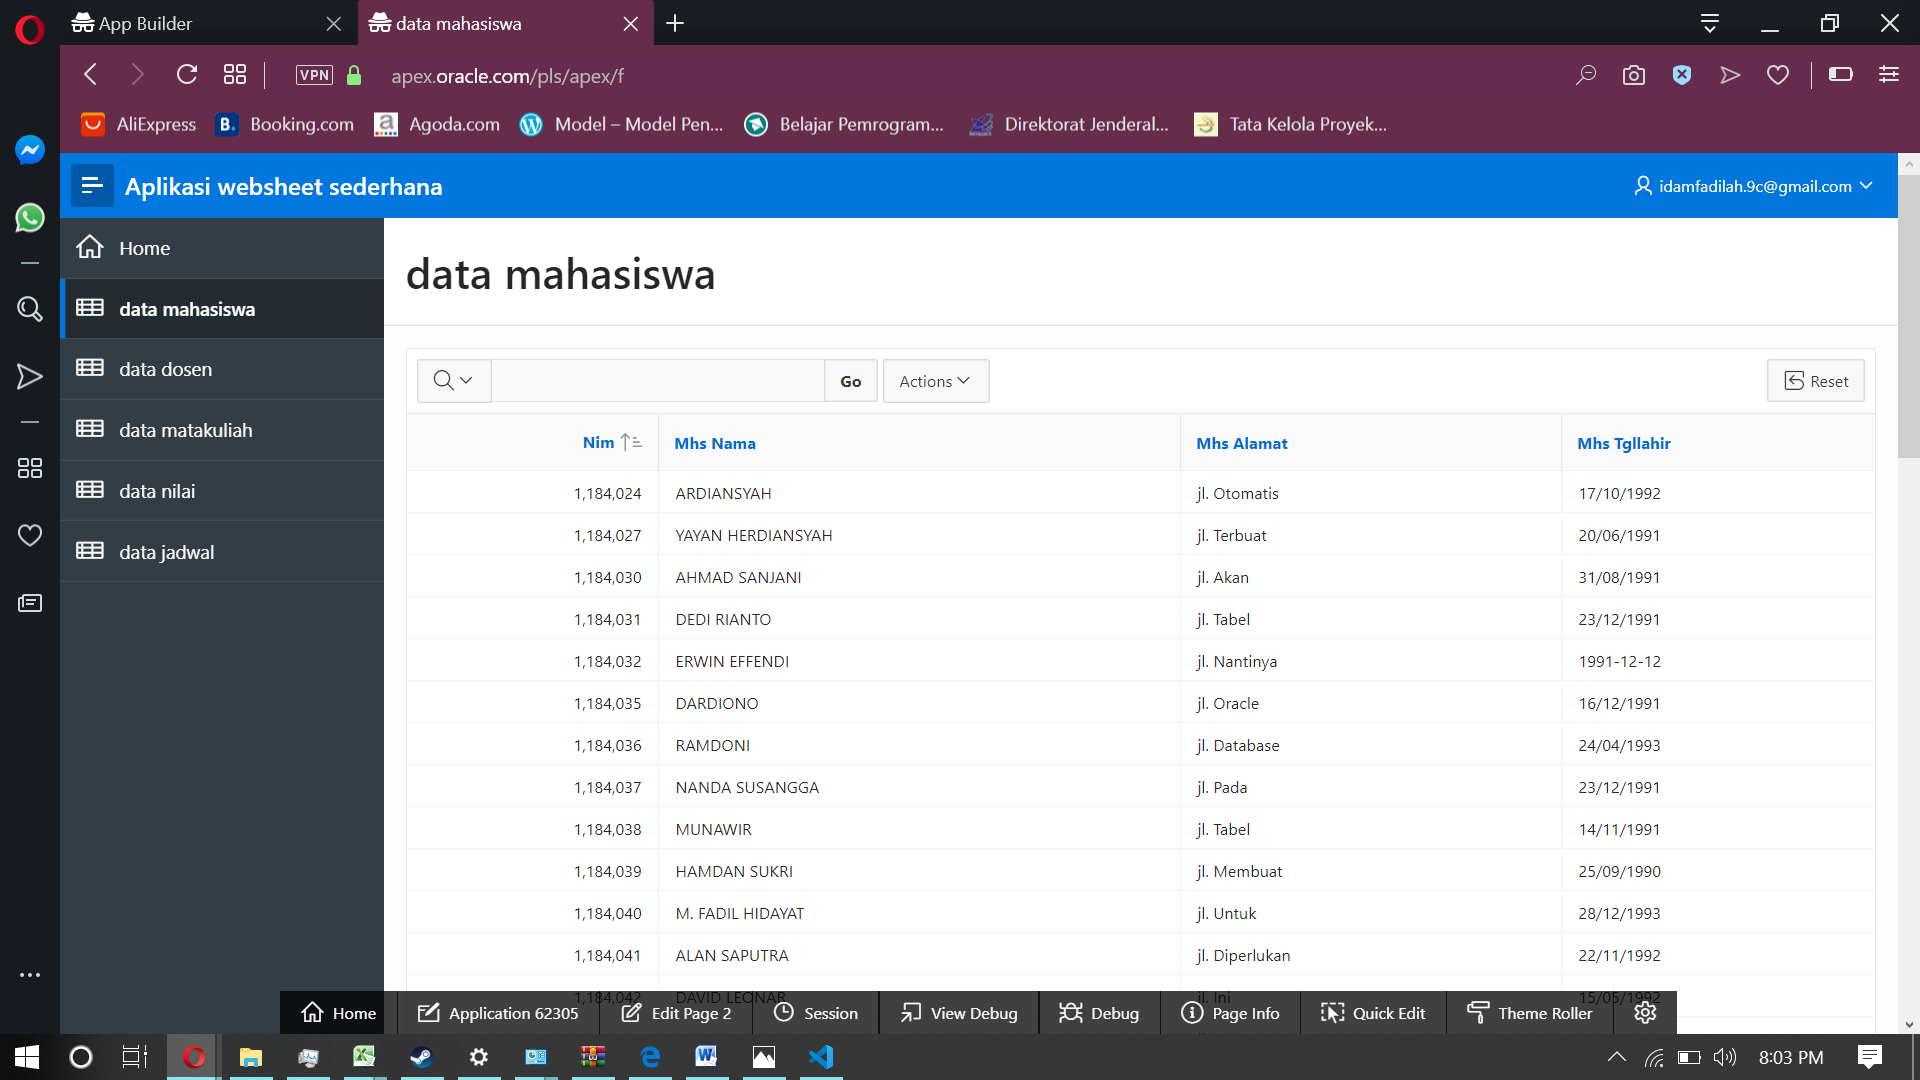
\includegraphics[width=10cm]{aplikasi websheet/Screenshot (170).png}\\
	

\end{itemize}
Workspace : tgsdb2\\
username  : idamfadilah.9c@gmail.com\\
password  : jcj223vi35\\
\end{document}
